\UseRawInputEncoding
%% Proxy4Tun — Automation in Construction (cas-dc double-column template)
%% Publication draft, 15 Sep 2026. Derived from Proxy4Tun_journal_revision-2026-09-14-205925.tex.

\documentclass[a4paper,fleqn]{cas-dc}

\usepackage[numbers]{natbib}
\usepackage{booktabs}
\usepackage{array}
\newcolumntype{L}[1]{>{\raggedright\arraybackslash}p{#1}}
\usepackage{multirow}
\usepackage{amsmath}
\usepackage{algorithm}
\usepackage{algpseudocode}
\usepackage{graphicx}
\usepackage[dvipsnames,table]{xcolor}
\usepackage{xurl}
\usepackage{hyperref}
\usepackage[nameinlink,noabbrev]{cleveref}
\usepackage{placeins}
\usepackage{caption}
\usepackage{float}
\usepackage{tikz}
\usetikzlibrary{shapes.geometric,arrows.meta,positioning,fit,calc}
\usepackage{listings}
\lstset{
  basicstyle=\ttfamily\footnotesize,
  breaklines=true,
  columns=fullflexible,
  frame=single,
  framesep=4pt,
  xleftmargin=0.5em,
  xrightmargin=0.5em,
  aboveskip=0.6em,
  belowskip=0.6em,
}

\providecommand{\printorcid}{}
\providecommand{\printfacebook}{}
\providecommand{\printtwitter}{}
\providecommand{\printlinkedin}{}
\providecommand{\printgplus}{}
\providecommand{\printinstagram}{}
\providecommand{\printemails}{}
\providecommand{\printurls}{}

\begin{document}
\let\WriteBookmarks\relax
\def\floatpagepagefraction{1}
\def\textpagefraction{.001}

% ────────────────────────────── Front matter ──────────────────────────────

\shorttitle{Proxy4Tun: proxy-driven quality control for point-cloud tunnel-lining segmentation}
\shortauthors{X.\ Tao et~al.}

\title[mode=title]{\texorpdfstring{Proxy4Tun: proxy-driven quality control for point-cloud tunnel-lining segmentation}{Proxy4Tun: proxy-driven quality control for point-cloud tunnel-lining segmentation}}

\author[1]{Xinghui Tao}
\credit{Conceptualization, Methodology, Software, Writing -- original draft}

\author[2]{Zehao Ye}

\author[1]{Guangming Wang}
\cormark[1]
\ead{gw462@cam.ac.uk}
\credit{Supervision, Writing -- review \& editing}

\author[2]{Jelena Nini\'{c}}
\credit{Supervision, Writing -- review \& editing}

\author[1]{Brian Sheil}
\credit{Supervision, Funding acquisition, Project administration, Writing -- review \& editing}

\cortext[cor1]{Corresponding author}

\affiliation[1]{organization={Construction Engineering, University of Cambridge},
    addressline={Trumpington Street},
    city={Cambridge},
    postcode={CB2 1PZ},
    country={United Kingdom}}

\affiliation[2]{organization={Department of Engineering, Durham University},
    addressline={Stockton Road},
    city={Durham},
    postcode={DH1 3LE},
    country={United Kingdom}}

% ─── Abstract (AIC limit: 150 words) ─────────────────────────────────────

\begin{abstract}
Segmenting tunnel-lining point clouds needs quality control when new scans arrive without ground-truth (GT) labels. Proxy4Tun estimates segmentation accuracy from intermediate pipeline measurements and uses the estimate to compare bounded parameter proposals. A four-feature Ridge proxy, calibrated on 120 trials from one labelled subset per Seg2Tunnel family and then frozen, is tested on 54 reference/degraded runs from 27 other subsets: Spearman 0.817, MAE 0.109, all 27 pairs ranked correctly, three false alarms. On 22 proxy-admitted cases, three LLM arms and a sparsity-matched random-overlay control share one GT-blind selector; selected mIoU rises from 0.738 to 0.759--0.768 (LLMs) and 0.752 (random). Unselected random proposals fall to about 0.53, so the selector supplies most of the gain; LLM edges over random are small with intervals that include zero. Claims are graded by evidence quality and confidence. The proxy is an auditable control signal, not an acceptance criterion or LLM ranking.
\end{abstract}

% ─── Highlights (3–5 bullets, ≤85 characters each) ───────────────────────

\begin{highlights}
\item Four-feature proxy ranks all 27 reference/degraded pairs on scans unseen in fitting.
\item Calibration needs one labelled subset per lining family and 120 parameter trials.
\item GT-blind selection lifts three LLM arms to 0.759--0.768 and random to 0.752 mIoU.
\item Selector filters harmful random proposals; LLM edges over random remain uncertain.
\item Every claim is graded by sensitivity analysis, evidence quality, and confidence.
\end{highlights}

% ─── Keywords ─────────────────────────────────────────────────────────────
\begin{keywords}
Segmental tunnel lining \sep Point cloud segmentation \sep Quality control \sep Label-free quality estimation \sep Parameter refinement \sep Large language models
\end{keywords}
\date{\today}

\maketitle

% ═════════════════════════════════════════════════════════════════════════
\section{Introduction}
\label{sec:intro}

Regular inspection of segmental tunnel linings supports structural health assessment and operational safety, and laser scanning captures the lining surface as a 3D point cloud quickly enough to make network-scale inspection practical~\cite{attard2018,montero2015,strauss2020sensing,huang2021bim,sjolander2023towards,weidner2024generalized}. Most downstream inspection tasks first require assigning each point to its lining block. Segmentation accuracy, however, changes with lining geometry, joint layout, occlusion, and scan quality, and checking every new output against manual labels or re-tuning parameters by hand is a recurring cost. Practitioners need to decide whether an output is accurate enough to accept, should be refined, or must be flagged for human review, without new ground-truth (GT) labels (Fig.~\ref{fig:deployment_qc_gap}).

\begin{figure*}[t]
\centering

\includegraphics[width=0.8\textwidth]{figs/motivation.pdf}
\caption{Deployment quality-control (QC) gap: segmentation methods produce candidate outputs, but practitioners must still decide whether to accept, refine, or flag each result. Without new GT labels this decision needs other evidence about accuracy.}
\label{fig:deployment_qc_gap}
\end{figure*}

Current approaches answer this need only partly. Geometric pipelines designed by engineers offer interpretable rules but must be retuned by hand when conditions change~\cite{huang2021bim,weidner2024generalized,wang2025automated}. Supervised networks can be retrained and may emit confidence scores, but those scores must be checked against actual accuracy before they can support QC~\cite{su2024review,cha2024deep}. Foundation-model pipelines reduce per-project annotation and expose prompts and preprocessing parameters for adaptation~\cite{bommasani2021foundation,kirillov2023sam,ye2024sam}, yet the ability to change a pipeline says nothing about whether the changed output is better. In medical imaging, segmentation quality has been estimated without GT for the new case by learning from labelled development data or by comparing against labelled references~\cite{valindria2017rca,robinson2018segmentationQuality,fournel2021segmentationQC}; whether this transfers to tunnel point-cloud pipelines, where annotations are scarce and processing depends on expert reference configurations, is open.

This paper asks whether measurements produced \emph{during} tunnel segmentation can be calibrated on a small labelled subset and an expert reference configuration per lining family, and then used to estimate accuracy and guide parameter refinement on unseen scans without new GT labels. Proxy4Tun answers this in three steps. Parameter trials on one labelled development subset per family generate segmentations of varying accuracy; a compact linear proxy is fitted to relate intermediate measurements, preprocessing quality (PQ) and structure coherence (SC), to GT mean intersection-over-union (mIoU) and is then frozen; and the frozen proxy is used to rank the outputs of bounded parameter proposals from three LLM proposal systems and a sparsity-matched random-overlay control under one shared GT-blind selector.

The contributions are:
\begin{enumerate}
\item A deployment-time accuracy proxy for tunnel-lining segmentation that combines PQ and SC measurements and is calibrated from limited offline annotations.
\item A frozen evaluation that separates numerical fidelity, pairwise ranking, and alarm performance on scans excluded from proxy fitting, with sensitivity analyses of its uncertainty.
\item A proxy-guided refinement study in which three LLM proposal systems and a random-overlay control share one selector, separating the value of proxy-based selection from proposer identity, and an explicit grading of the evidence behind each claim.
\end{enumerate}

Throughout, GT labels support offline calibration and evaluation only; the scorer, the selector, and every proposal prompt exclude them. One annotation-derived input remains upstream: the evaluated pipeline reads the dataset's per-point ring index to orient and validate the unfolded coordinate frame (Section~\ref{sec:pipeline}). The paper therefore claims GT-blind scoring and selection, not end-to-end annotation-free execution.

% ═════════════════════════════════════════════════════════════════════════
\section{Related work}
\label{sec:related}

\paragraph{Tunnel segmentation and adaptation.}
Geometric pipelines identify lining surfaces and joints from rules and thresholds that must be adjusted when geometry or scan quality changes~\cite{huang2021bim,weidner2024generalized,wang2025automated}. Supervised point-cloud networks, from PointNet++ and RandLA-Net to instance-level Mask3D and TD3D and the tunnel-specific LiningNet, learn from labelled scans but need new annotations and retraining under substantially different conditions~\cite{qi2017pointnet,hu2020randla,schult2023mask3d,kolodiazhnyi2024td3d,lin2025liningnet,su2024review,cha2024deep}. Prompt-based foundation models (SAM, SAM2, SEEM) have been applied to crack segmentation and Scan-to-BIM~\cite{kirillov2023sam,ravi2024sam2,zou2023segment,ge2024cracksam,ye2024sam,wang2024omni,pan2024zero,ye2026maintenance}; SAM4Tun unfolds tunnel point clouds into panoramas and prompts SAM from a lining template without task-specific training~\cite{ye2025sam4tun}, but its preprocessing and prompting parameters still encode assumptions about geometry and scanning. R4Tun lets an LLM propose bounded adjustments to those parameters from reference information and intermediate outputs~\cite{taoR4Tun}; it does not assess the accuracy of the initial or adjusted output without GT, which is the gap addressed here.

\paragraph{Quality estimation without new GT labels.}
Segmentation quality has been predicted from features of the image and the segmentation~\cite{kohlberger2012evaluating,robinson2018segmentationQuality}, from input features and network confidence for LiDAR segments~\cite{colling2021lidarmetaseg}, and from agreement between processing streams, although agreement can be jointly wrong~\cite{bogdoll2025labelfree}. Reference-based methods such as Reverse Classification Accuracy and its in-context variant estimate quality by evaluating the new segmentation against labelled reference cases~\cite{valindria2017rca,cosarinsky2026conficrca}. Proxy4Tun follows the first family: it scores a run from its own measurements and an expected ring count, without comparing against reference-run measurements, and it tests whether the learned relationship persists on unseen scans.

\paragraph{Calibration with limited labels.}
Varying model settings on a labelled input yields many segmentations of different quality from the same annotation~\cite{robinson2018segmentationQuality}. Bayesian optimisation with priors (BOPrO, $\pi$BO) and space-filling designs guide which settings to evaluate~\cite{souza2020prior,hvarfner2022pibo,joe2008constructing}, and Gaussian-process uncertainty can direct further evaluations to poorly covered regions~\cite{gramacy2009adaptive,gramacy2020surrogates}. We use these tools to collect examples that span successful and degraded outputs around an expert reference, rather than to search for the optimum.

\paragraph{Feedback-guided refinement.}
Self-Refine, Reflexion, AlphaEvolve, and the Darwin G\"odel Machine revise outputs or programs from feedback~\cite{madaan2023selfrefine,shinn2023reflexion,novikov2025alphaevolve,zhang2025darwin}, but self-correction without external feedback can fail, and optimising an imperfect proxy can reduce true performance~\cite{huang2024selfcorrect,gao2023overoptimization}. ReAct shows how observations inform the next action~\cite{yao2023react}, and interpretable models make a score's composition auditable~\cite{rudin2019stop}. Proxy4Tun supplies PQ and SC measurements as diagnostic observations and a linear score as the comparison signal, and it retains the starting run so that a proxy-guided loop cannot lower the proxy score; whether it can lower true accuracy is one of the questions tested.

% ═════════════════════════════════════════════════════════════════════════
\section{Methodology}
\label{sec:methods}

Proxy4Tun separates offline calibration from deployment (Fig.~\ref{fig:intrinsic_proxy_scoring}). Parameter trials on labelled development scans establish how pipeline measurements relate to accuracy; the fitted proxy is frozen; and at deployment it scores new outputs and ranks bounded parameter proposals.

\begin{figure*}[t]
\centering

\includegraphics[width=\textwidth]{figs/intrinsics.pdf}
\caption{Development and use of the accuracy proxy. Parameter variations produce outputs of different accuracy; PQ and SC measurements paired with GT mIoU train the proxy. Once frozen, it estimates accuracy on new runs from measurements available without GT. The score is an estimate, not a guarantee.}
\label{fig:intrinsic_proxy_scoring}
\end{figure*}

\subsection{Task and pipeline}
\label{sec:pipeline}

The segmentation task assigns each point to a positional lining-block class (key block K, adjacent blocks B1/B2, standard blocks A1--A$n$; Fig.~\ref{fig:task}) or to background. A ring holds six blocks in the staggered and continuous families and seven in the complex family; ring membership is recorded but is not part of the semantic metric. The assessment task is to estimate, for a completed run on a multi-ring subset, its GT mIoU from intermediate outputs and the expected ring count only.

\begin{figure*}[t]
\centering
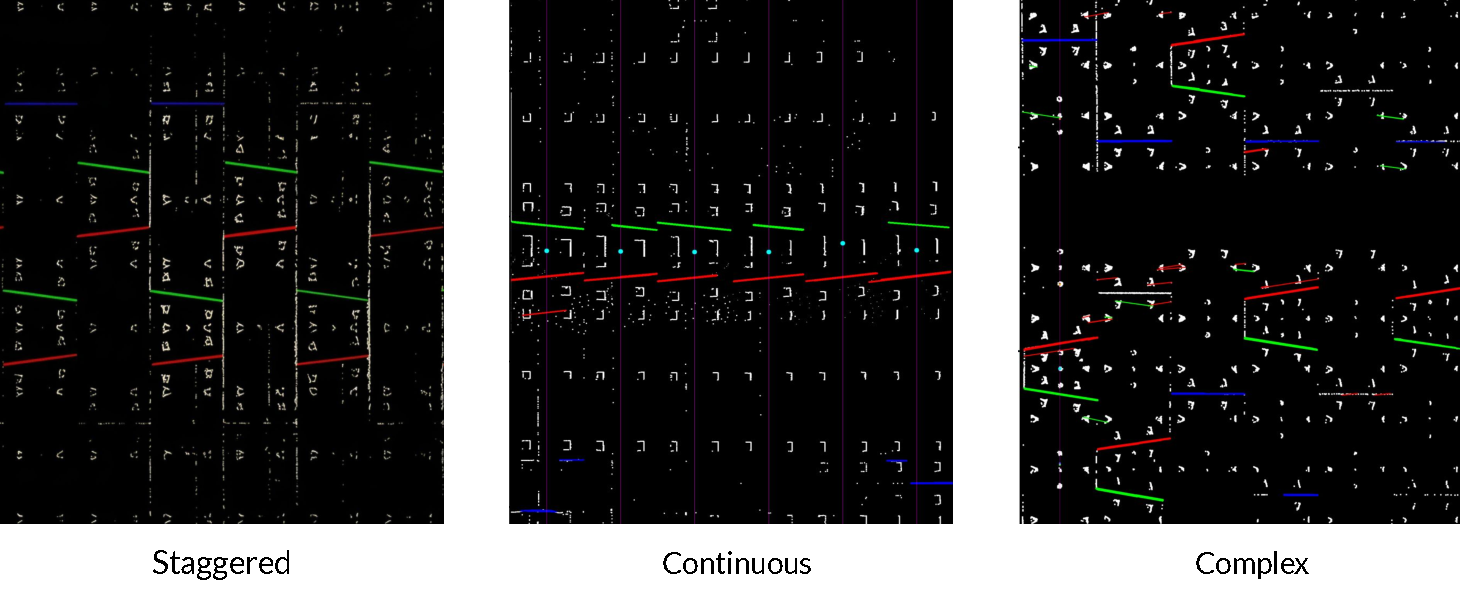
\includegraphics[width=0.8\textwidth]{figs/task.pdf}
\caption{Lining block types: key (K), adjacent (B), and standard (A) blocks, with background labelled separately.}
\label{fig:task}
\end{figure*}

The pipeline is adapted from SAM4Tun~\cite{ye2025sam4tun} and has five deployable stages (Fig.~\ref{fig:pipeline}): (1)~\emph{unfolding}, RANSAC ellipse fitting and centreline estimation define cylindrical coordinates and a depth panorama~\cite{fischler1981ransac}; (2)~\emph{denoising}, radial gates and density filtering remove off-lining points~\cite{ester1996dbscan}; (3)~\emph{enhancement}, curvature-guided interpolation and upsampling complete the depth map; (4)~\emph{boundary detection}, orientation-specific Hough transforms find ring and block joints~\cite{duda1972hough}; (5)~\emph{segmentation}, the detected layout defines template prompts for SAM~\cite{kirillov2023sam}, and masks are reprojected onto the points. A GT-dependent evaluation step runs offline only and has no parameters. Stage algorithms and SAM weights are fixed; exploration and refinement change only parameters. Each family has an expert \emph{reference configuration}; a proposal is an overlay listing the parameters to change, applied to a recorded base configuration (Appendix~\ref{app:anchor-parameter}).

\begin{figure*}[t]
\centering

\includegraphics[width=0.98\textwidth]{figs/pipeline.pdf}
\caption{Segmentation pipeline adapted from SAM4Tun. Intermediate outputs of each stage supply the PQ and SC measurements. Stage algorithms are fixed; only parameters change.}
\label{fig:pipeline}
\end{figure*}

Two conventions matter for what follows. First, stage~1 fixes the coordinate frame using the per-point ring index stored in the Seg2Tunnel files~\cite{lin2024seg2tunnel}: the centreline direction is chosen so that the axial coordinate correlates with the ring index with a prescribed sign, and the stage aborts unless the Pearson correlation exceeds 0.5 in magnitude. This index is a distributed ring annotation, not sensor metadata. It contributes one binary orientation choice and one validity check per subset, is never passed to the scorer or proposer, and reads no semantic label; but it shapes the frame on which all measurements are computed, so the executed pipeline is annotation-assisted at stage~1 (Appendix~\ref{app:anchor-parameter}). Second, stage-1 parameters are locked during refinement unless the starting run's recentring residual exceeds 10\,cm, so that candidate outputs of one case share a frame.

\subsection{Calibration examples}
\label{sec:bo-experience}

Calibration needs examples that link measurements to accuracy under both successful and degraded settings. For each family, one labelled development subset is processed under 40 parameter settings within expert-prescribed bounds: 32 valid scrambled-Sobol trials for coverage~\cite{joe2008constructing}, then eight valid trials placed where a Gaussian-process model of GT mIoU is most uncertain~\cite{gramacy2009adaptive,gramacy2020surrogates}. All runs on a subset are scored against the same annotation, so additional runs cost computation, not labelling. A trial is valid when all stages complete and all ten candidate measurements are finite; 121 trials were attempted and one failed. Each valid run records its parameters, measurements, and GT mIoU, giving 120 records. The acquisition targets uncertainty rather than high accuracy, so the records deliberately include poor outputs (GT mIoU from about 0.03 upward). Appendix~\ref{app:bo-config} gives the sampler, GP configuration, and bounds.

\subsection{Measurements and proxy}
\label{sec:features}

Ten candidate measurements are computed from each run without its GT labels (Table~\ref{tab:candidate-features}). PQ measurements describe the completeness and geometric plausibility of the representation supplied to later stages: depth-map completeness, point support, and alignment. SC measurements describe whether the recovered layout is coherent: agreement between detected joints and predicted label boundaries, coverage, label consistency across rings, and the \emph{ring-count residual} $|N_{\mathrm{det}}-N_{\mathrm{exp}}|$. Here $N_{\mathrm{exp}}$ (ten in these experiments) is a design or acquisition prior, not a segmentation label: the residual flags layout-count mismatch as one coherence check alongside correspondence and fill, and does not imply that ring count alone determines accuracy. A hard count gate remains available operationally; the proxy keeps the residual as a graded term. Because joint detections also drive SAM prompting, joint--boundary agreement can share correlated errors with the segmentation; it is evidence, not proof, of correctness.

\begin{table*}[t]
\caption{Candidate measurements for the accuracy proxy (four PQ, six SC). Pixel quantities refer to the 5\,mm depth-image grid. The four retained by the frozen proxy are marked $\star$ and defined in Eqs.~\eqref{eq:feature-defs}--\eqref{eq:corr-f1}.}
\label{tab:candidate-features}
\centering
\small
\setlength{\tabcolsep}{3pt}
\begin{tabular}{L{0.05\textwidth} L{0.27\textwidth} L{0.45\textwidth} L{0.16\textwidth}}
\toprule
Group & Measurement & Meaning & Stage \\
\midrule
PQ & Unfolding fit residual & Centreline fit error & 1 \\
 & Orientation agreement & Difference between inferred and expected axes & 1 \\
 & Point retention & Fraction of input points kept after denoising & 2 \\
 & Missing-depth rate $\star$ & Fraction of depth-image pixels without depth after enhancement & 3 \\
SC & Ring-count residual $\star$ & $|N_{\mathrm{det}}-N_{\mathrm{exp}}|$ vs design/acquisition prior (stored as \texttt{ring\_count\_error}) & 4 \\
 & Edge support & Fraction of label-boundary pixels within 25\,px of a depth edge & 3+5 \\
 & Correspondence score $\star$ & F1 between detected joint lines and predicted block boundaries at 15\,px & 4+5 \\
 & Line--boundary distance & Symmetric mean distance (capped at 200\,px) between joints and boundaries & 4+5 \\
 & Fill rate $\star$ & Fraction of input points assigned a non-background label & 5 \\
 & Phase incoherence & Inconsistency of label ordering across rings & 5 \\
\bottomrule
\end{tabular}
\end{table*}

Let $\Omega$ be the depth-image grid (5\,mm pixels), $V\subseteq\Omega$ the pixels with defined depth, $\mathcal P$ the input points, $\ell(p)$ the predicted label of point $p$ (0 for background, including points removed by denoising), and $N_{\mathrm{det}}$ the number of ring columns detected in stage~4. The four retained measurements are
\begin{equation}
\begin{aligned}
x_{\mathrm{nan}}&=\frac{|\Omega\setminus V|}{|\Omega|},\\
x_{\mathrm{ringerr}}&=|N_{\mathrm{det}}-N_{\mathrm{exp}}|,\\
x_{\mathrm{fill}}&=\frac{|\{p\in\mathcal P:\ell(p)>0\}|}{|\mathcal P|},
\end{aligned}
\label{eq:feature-defs}
\end{equation}
where $x_{\mathrm{ringerr}}$ is the ring-count residual. The correspondence score $x_{\mathrm{corr}}$ is an F1 between the rasterised detected joint lines $L$ and the pixels $B$ where two different non-background labels meet circumferentially within a predicted ring. With $d(\cdot,S)$ the distance transform to $S$ and $\delta=15$\,px (75\,mm),
\begin{equation}
\begin{aligned}
\pi_\delta&=\frac{|\{u\in L: d(u,B)\le\delta\}|}{|L|},\\
\gamma_\delta&=\frac{|\{u\in B: d(u,L)\le\delta\}|}{|B|},\\
x_{\mathrm{corr}}&=\frac{2\pi_\delta\gamma_\delta}{\pi_\delta+\gamma_\delta},
\end{aligned}
\label{eq:corr-f1}
\end{equation}
with an empty set giving its fraction 0 and $x_{\mathrm{corr}}=0$ when $\pi_\delta+\gamma_\delta=0$, so severe disagreement scores the finite worst value. A run whose four measurements are not all finite is unscorable and is recorded as a failure, never imputed. Tolerances of 8 and 25\,px change LOFO correlation by less than 0.01 (Appendix~\ref{app:proxy-package}).

The proxy is a Ridge regression on standardised measurements~\cite{hoerl1970ridge,pedregosa2011sklearn},
\begin{equation}
\hat y(\mathbf x)=b+\sum_{j} w_j\frac{x_j-\mu_j}{s_j},
\label{eq:ridge-proxy}
\end{equation}
with the penalty chosen from 25 log-spaced values in $[10^{-3},10^{3}]$ by leave-one-out cross-validation on the fitting data and predictions clipped to $[0,1]$ (no evaluation prediction required clipping). The linear form makes each measurement's contribution explicit. Feature sets are compared by leave-one-family-out (LOFO) validation: fit on two families (80 runs), test on the third (40), with scaling and penalty chosen inside the training split. The compact set was selected among eight nested candidates (top-$k$ features by standardised coefficient, $k=3,\ldots,10$, plus the set of coefficients above 10\% of the largest) by LOFO Spearman correlation. Because held-out folds were used to choose the set, LOFO figures are model-selection diagnostics; the frozen 27-subset test of Section~\ref{sec:stress-test} is the unbiased estimate. The selected four-feature model was refitted on all 120 records and frozen before any evaluation-panel scoring (Appendix~\ref{app:proxy-package}). A permutation control shuffles GT mIoU within family (20 repeats) and refits, to check that the association is not driven by family means.

\subsection{Proxy-guided refinement}
\label{sec:agent-design}

The refinement loop (Fig.~\ref{fig:verification}) is proposer-agnostic; here the proposer is either an LLM agent that receives the current settings, intermediate outputs, the four measurements and stage-1 residual, previous proxy feedback, the family reference, and a structured engineering ontology of failure modes, permitted changes, and stage dependencies (Appendix~\ref{app:panel-config}), or a sparsity-matched random-overlay sampler that draws bounded overlays without that context. Each admitted case receives three attempts; an attempt returns one overlay, which is validated against the family search space (names, types, marginal bounds; stage-1 keys only when unlocked), executed through stages~1--5, measured, and scored. Invalid or failed attempts are recorded and excluded from selection; there is no early stopping.

Admission uses the proxy score of the starting run once, before the loop, through the study operating bands
\begin{equation}
\operatorname{QC}(\hat y)=
\begin{cases}
\text{flag}, & \hat y<0.5,\\
\text{refine}, & 0.5\le\hat y<0.7,\\
\text{accept}, & \hat y\ge0.7,
\end{cases}
\label{eq:qc-bands}
\end{equation}
which illustrate assessment decisions and are not validated engineering acceptance criteria. Only ``refine'' starts enter the loop.

Selection is monotone in the proxy and keeps the start eligible. Let $r=0$ be the start, $\mathcal V$ the scored candidates, $\hat y_r$ the clipped score, and $\eta_r$ the stage-1 recentring residual (cm). With $\mathcal C=\{r\in\mathcal V:\hat y_r>\hat y_0\}$ and $\mathcal C_\varepsilon=\{r\in\mathcal C:\hat y_r\ge\max_{\mathcal C}\hat y-\varepsilon\}$, $\varepsilon=0.01$,
\begin{equation}
r^\star=
\begin{cases}
0, & \mathcal C=\emptyset,\\
\operatorname*{arg\,min}_{r\in\mathcal C_\varepsilon}(\eta_r,\,-\hat y_r), & \text{otherwise},
\end{cases}
\label{eq:refinement-selection}
\end{equation}
where the minimisation is lexicographic: among near-tied candidates the lower residual, then the higher score, is preferred. The residual is a GT-free stage-1 quantity used only as a tie-break. Because the complete rule produced the reported selections, Section~\ref{sec:poc-verification} also reports pure maximum-proxy selection to show how much the tie-break mattered. Algorithm~\ref{alg:reflective_adaptation} summarises the procedure.

\begin{algorithm}[!htb]
\caption{Proxy-guided parameter refinement}
\label{alg:reflective_adaptation}
\small
\begin{algorithmic}[1]
\Require Subset $D$; start $P_0$ (expert family reference); frozen proxy $g$; bounds; budget $R=3$; $\varepsilon=0.01$
\Ensure Retained configuration $P^\star$ and QC status
\State Execute $P_0$; if it fails or any measurement is non-finite, \Return $P_0$, flag
\State $\hat y_0\gets\operatorname{clip}(g(\mathbf x_0),0,1)$; $\eta_0\gets$ stage-1 residual
\If{$\hat y_0<0.5$ \textbf{or} $\hat y_0\ge0.7$} \Return $P_0$, $\operatorname{QC}(\hat y_0)$ \Comment{pre-loop return, Eq.~\eqref{eq:qc-bands}}
\EndIf
\State $\mathcal V\gets\emptyset$
\For{$r=1,\ldots,R$}
  \State Obtain overlay from the proposer (context: settings, outputs, measurements, scores, history)
  \State Validate overlay against bounds and stage-1 lock; \textbf{if} invalid, record and \textbf{continue}
  \State $P_r\gets\operatorname{Apply}(P_0,\text{overlay})$; run stages 1--5; \textbf{if} failure, record and \textbf{continue}
  \State $\hat y_r\gets\operatorname{clip}(g(\mathbf x_r),0,1)$; $\eta_r\gets$ residual; $\mathcal V\gets\mathcal V\cup\{r\}$
\EndFor
\State $r^\star\gets$ Eq.~\eqref{eq:refinement-selection}; $P^\star\gets P_{r^\star}$
\State \Return $P^\star$, $\operatorname{QC}(\hat y_{r^\star})$
\end{algorithmic}
\end{algorithm}

\paragraph{Information boundary.}
The scorer reads only the four measurements of the run being scored; the selector reads only proxy scores and residuals; and no GT label, GT value, or evaluation file of the scan under refinement is placed in any proposal prompt. Two qualifications apply. Upstream, stage~1 uses the ring-index annotation as described in Section~\ref{sec:pipeline}. Experimentally, the three proposer arms differ in context history: GPT-5.6 and Gemini~3.8 ran in fresh per-case contexts, whereas the Fable~5.1 session had earlier been exposed to aggregate pilot evaluation summaries and to the GT-band membership of six cases (Section~\ref{sec:poc-protocol}). Excluding GT from the current prompt is therefore not equivalent to a sanitised session history for that arm.

\subsection{Experimental design}
\label{sec:exp-setup}

\subsubsection{Data and use of annotations}
\label{sec:dataset}

We use Seg2Tunnel subsets from three lining families~\cite{lin2024seg2tunnel} (Table~\ref{tab:dataset}). Subsets 2-1, 3-1, and 5-1 are the development subsets and supply the 120 calibration records. The evaluation panel comprises 27 other subsets, nine per family, all excluded from proxy fitting. ``Held out'' refers to proxy calibration only: the expert reference configurations for 1-1 and 4-1 were tuned on those scans' own GT and then reapplied to them, whereas the other 25 subsets receive reference settings established on a different scan of the same tunnel. Every stage-1 execution reads the ring-index annotation for frame orientation. The degraded overlays for the continuous and complex families were identified by GT from earlier exploration trials on evaluation subsets 3-2 and 4-1 (Section~\ref{sec:stress-test}). Evaluation labels are otherwise used only to measure performance and to define retrospective GT strata.

\begin{table*}[t]
\caption{Calibration and evaluation subsets, and every use of annotation-derived information. All 27 evaluation subsets are excluded from proxy fitting.}
\label{tab:dataset}
\centering
\small
\setlength{\tabcolsep}{4pt}
\begin{tabular}{L{0.20\textwidth} L{0.22\textwidth} L{0.22\textwidth} L{0.26\textwidth}}
\toprule
Property & Staggered (T1, T2) & Continuous (T3) & Complex (T4, T5) \\
\midrule
Inner diameter / ring length & 5.5\,m / 1.2\,m & 5.9\,m / 1.2\,m & 7.5\,m / 1.8\,m \\
Blocks per ring; key layout & 6; ring-to-ring repeating & 6; fixed ring-wise order & 7; no repeating pattern \\
Scanning & Single-station & Multi-station & Single-station, offset \\
Development subset (40 runs) & 2-1 & 3-1 & 5-1 \\
Evaluation subsets & 1-1--1-5; 2-2--2-5 & 3-2--3-10 & 4-1--4-5; 5-2--5-5 \\
Reference source per tunnel & 1-1 (own GT); 2-1 & 3-1 profile & 4-1 (own GT); 5-1 \\
Degraded-overlay source (GT mIoU) & 2-1 trial (0.032) & 3-2 trial (0.027) & 4-1 trial (0.036) \\
\midrule
\multicolumn{4}{p{0.94\textwidth}}{Additional uses: every stage-1 run reads the ring-index annotation for frame orientation and validation; the Fable~5.1 session was exposed to aggregate pilot evaluation summaries and to the GT-band membership of 1-4, 1-5, 2-2, 3-4, 4-1, and 4-3 before its reported proposals (Section~\ref{sec:poc-protocol}).} \\
\bottomrule
\end{tabular}
\end{table*}

\subsubsection{Paired degradation test}
\label{sec:stress-test}

Each evaluation subset is processed with its unmodified reference configuration and with a degraded counterpart. The degradation rule was fixed before the proxy was frozen: for each family, the lowest-mIoU completed trial in an earlier parameter-exploration archive supplies a stage-2--5 overlay (Appendix~\ref{app:anchor-parameter}), applied unchanged on top of every subset's reference; stage-1 settings are inherited so that both members share a frame, and the full pipeline is rerun. No label or boundary is edited directly. This gives 27 pairs and 54 runs, all of which executed and were scorable. Because one overlay per family is reused on nine scans, the degraded runs represent three severe parameter failure modes (GT mIoU 0.03--0.12), not 27 independent or marginal failures; the test measures discrimination under these perturbations, not operational false-alarm rates.

\subsubsection{Refinement panel and proposal arms}
\label{sec:poc-protocol}

The starting run of every evaluation subset is its reference run. The 22 starts with $0.5\le\hat y_0<0.7$ form the refinement panel; three starts fall below and two above the band, and GT plays no part in admission. Each case receives three proposals from each of three LLM proposal systems, Fable~5.1, GPT-5.6, and Gemini~3.8, and from a fourth \emph{random-overlay} control arm, under an identical proxy, validator, budget, execution code, and selector (Appendix~\ref{app:panel-config}). All $264$ proposals ($22\times3\times4$) executed. Stage~1 was unlocked in four cases (3-4, 3-8, 3-10, 4-3).

The LLM arms are \emph{session-attributed proposal systems}, not verified model interventions. Model identifiers come from agent-interface sessions, not provider API records; decoding settings were not controllable; and the arms differ in context history. Fable~5.1 ran in one persistent session in which six cases (1-4, 1-5, 2-2, 3-4, 4-1, 4-3), selected by both the proxy band and the GT band $[0.5,0.7)$, had been refined first in a pilot; their stored proposals are reused, and the remaining 16 cases were processed afterwards in the same session. Per-case GT was never placed in a prompt, but session-level exposure to aggregate evaluation summaries and to that cohort's membership cannot be excluded as an influence. GPT-5.6 and Gemini~3.8 used fresh per-case contexts, although not every later proposal is demonstrably conditioned on the preceding execution (for Gemini~3.8 most cases had all three proposals prepared before execution). The LLM comparison is therefore exploratory and compares realised proposal systems, not intrinsic LLM capability.

The random-overlay arm answers whether an LLM is needed at all as the proposer. For each case it draws three overlays non-adaptively (all three before any execution) with a fixed seed. The number of changed knobs $k$ is sampled from the pooled empirical distribution of knobs that the three LLM arms actually changed relative to the expert reference on the 198 panel records (excluding $k=0$); the chosen knobs then receive values drawn uniformly within the family search-space bounds, with the same integer, Boolean, and radial-gate repairs as the calibration sampler, and with unfolding knobs available only when stage~1 is unlocked. Values are not step-size matched to the LLMs; the control matches proposal sparsity, not proposal geometry. The same validator and selector then act on the executed candidates.

To separate the selector from the proposals, each arm is also summarised under reference policies applied to the same executed candidates: retain the start; always take round~1; a uniformly random round (reported as its expectation, the mean of the three rounds); pure maximum-proxy selection with the start eligible and no tie-break; and a GT oracle (best of start and three rounds). These are post-hoc fixed-pool comparisons; an adaptive proposer might have generated different later proposals under a different rule.

\begin{figure*}[t]
\centering
\resizebox{\textwidth}{!}{%
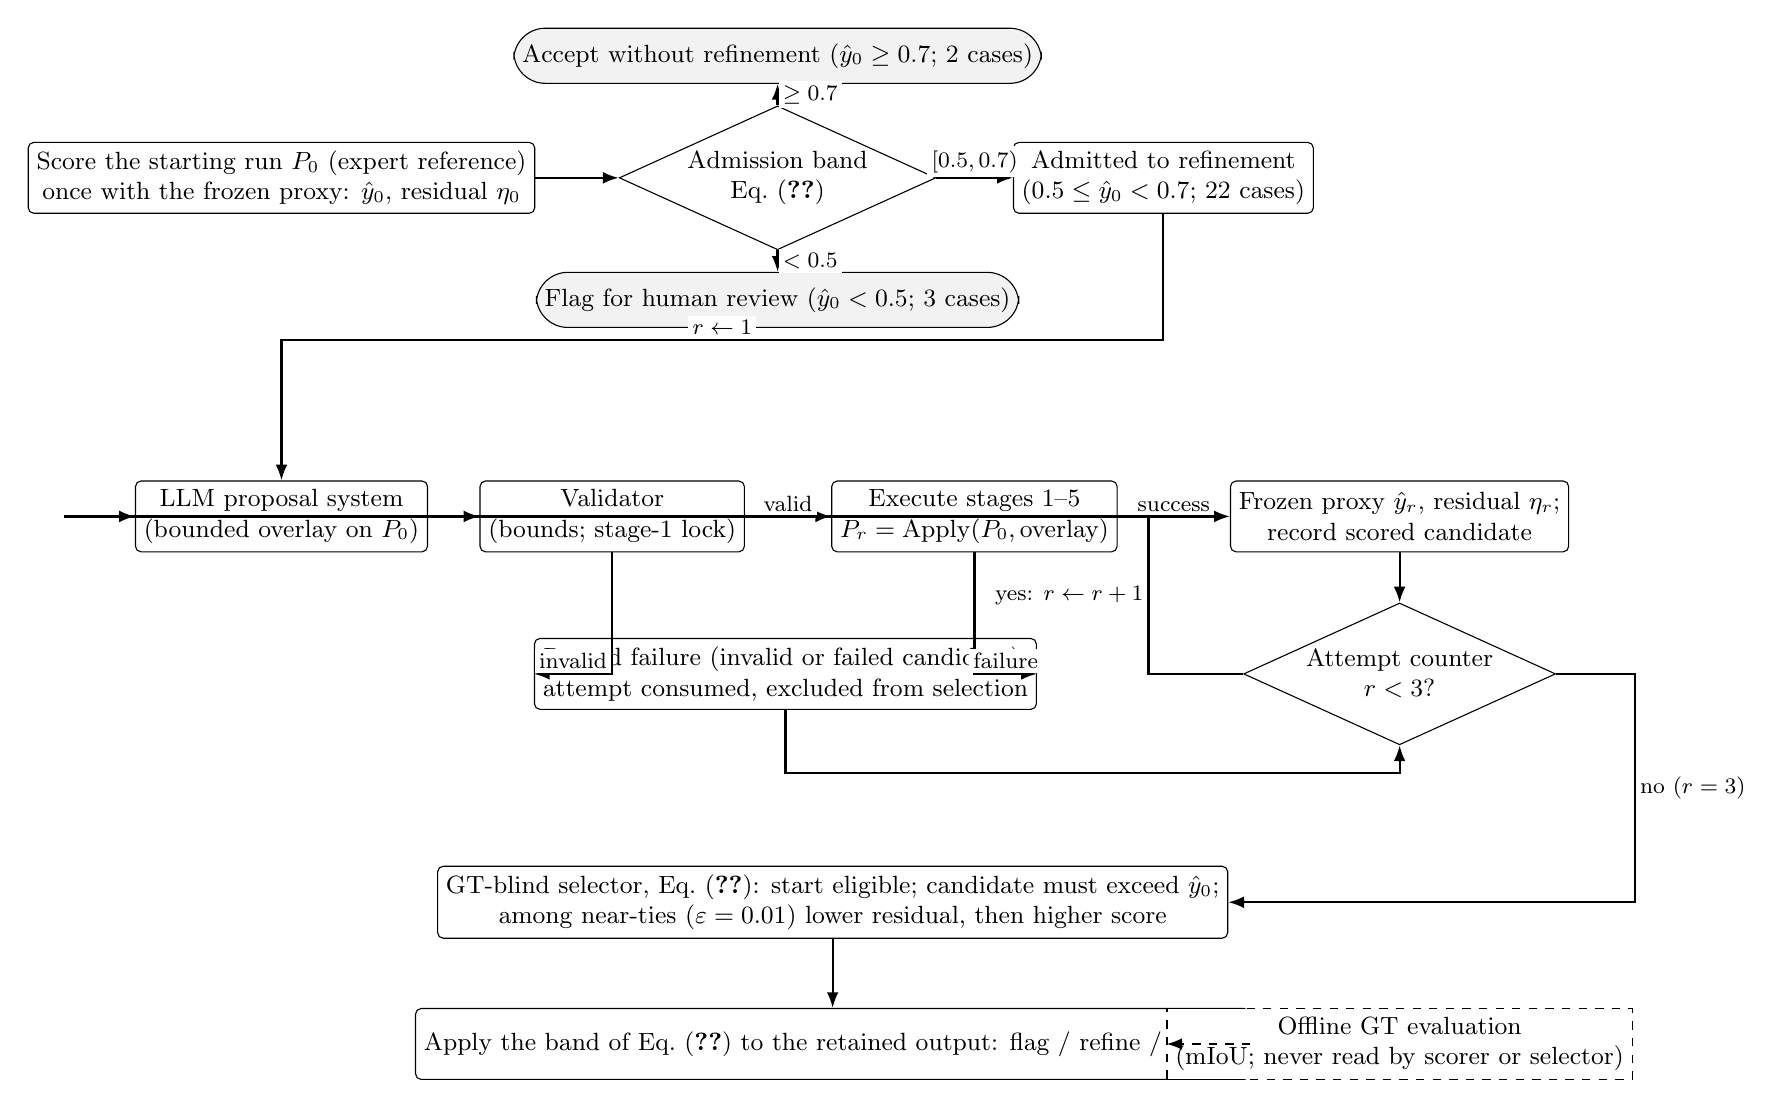
\begin{tikzpicture}[x=1cm,y=1cm,
  font=\small,
  box/.style={draw,rounded corners=2pt,align=center,minimum height=9mm,inner sep=3pt,fill=white},
  dec/.style={draw,diamond,aspect=2.2,align=center,inner sep=1pt,fill=white},
  term/.style={draw,rounded corners=4mm,align=center,minimum height=7mm,inner sep=3pt,fill=gray!10},
  gt/.style={draw,dashed,align=center,minimum height=8mm,inner sep=3pt,fill=white},
  arr/.style={-{Latex[length=2mm]},thick},
  lab/.style={font=\footnotesize,fill=white,inner sep=1.5pt}]
% ---------- Row 1: single admission decision ----------
\node[box] (score0) at (0,0) {Score the starting run $P_0$ (expert reference)\\once with the frozen proxy: $\hat y_0$, residual $\eta_0$};
\node[dec] (adm) at (6.3,0) {Admission band\\Eq.~\eqref{eq:qc-bands}};
\node[box] (admit) at (11.2,0) {Admitted to refinement\\($0.5\le\hat y_0<0.7$; 22 cases)};
\node[term] (acc0) at (6.3,1.55) {Accept without refinement ($\hat y_0\ge0.7$; 2 cases)};
\node[term] (flag0) at (6.3,-1.55) {Flag for human review ($\hat y_0<0.5$; 3 cases)};
\draw[arr] (score0) -- (adm);
\draw[arr] (adm.east) -- node[lab,above]{$[0.5,0.7)$} (admit.west);
\draw[arr] (adm.north) -- node[lab,right]{$\ge0.7$} (acc0.south);
\draw[arr] (adm.south) -- node[lab,right]{$<0.5$} (flag0.north);
% ---------- Row 2: fixed-budget loop ----------
\node[box] (prop) at (0,-4.3) {LLM proposal system\\(bounded overlay on $P_0$)};
\node[box] (val) at (4.2,-4.3) {Validator\\(bounds; stage-1 lock)};
\node[box] (exec) at (8.8,-4.3) {Execute stages 1--5\\$P_r=\operatorname{Apply}(P_0,\text{overlay})$};
\node[box] (scorer) at (14.2,-4.3) {Frozen proxy $\hat y_r$, residual $\eta_r$;\\record scored candidate};
\node[box] (fail) at (6.4,-6.3) {Record failure (invalid or failed candidate);\\attempt consumed, excluded from selection};
\node[dec] (cnt) at (14.2,-6.3) {Attempt counter\\$r<3$?};
\draw[arr] (admit.south) |- ($(admit.south)+(0,-1.6)$) -| node[lab,pos=0.25,above]{$r\gets1$} (prop.north);
\draw[arr] (prop) -- (val);
\draw[arr] (val) -- node[lab,above]{valid} (exec);
\draw[arr] (exec) -- node[lab,above]{success} (scorer);
\draw[arr] (val.south) |- node[lab,pos=0.75,above]{invalid} (fail.west);
\draw[arr] (exec.south) |- node[lab,pos=0.75,above]{failure} (fail.east);
\draw[arr] (scorer.south) -- (cnt.north);
\draw[arr] (fail.south) |- ($(fail.south)+(0,-0.8)$) -| (cnt.south);
\draw[arr] (cnt.west) -- ++(-1.2,0) |- node[lab,pos=0.25,left]{yes: $r\gets r+1$} ($(prop.west)+(-0.9,0)$) -- (prop.west);
% ---------- Row 3: selection ----------
\node[box] (sel) at (7.0,-9.2) {GT-blind selector, Eq.~\eqref{eq:refinement-selection}: start eligible; candidate must exceed $\hat y_0$;\\among near-ties ($\varepsilon=0.01$) lower residual, then higher score};
\node[box] (band) at (7.0,-11.0) {Apply the band of Eq.~\eqref{eq:qc-bands} to the retained output: flag / refine / accept};
\node[gt] (gtb) at (14.2,-11.0) {Offline GT evaluation\\(mIoU; never read by scorer or selector)};
\draw[arr] (cnt.east) -- ++(1.0,0) |- node[lab,pos=0.25,right]{no ($r=3$)} ($(sel.east)+(0.5,0)$) -- (sel.east);
\draw[arr] (sel) -- (band);
\draw[arr,dashed] (band.east) -- (gtb.west);
\end{tikzpicture}}
\caption{Refinement protocol. Top: the frozen proxy scores the starting run once and the band admits, accepts, or flags it. Middle: each of three attempts yields one bounded overlay that is validated, executed, and scored; failures consume an attempt. Bottom: the GT-blind selector chooses among the start and scored candidates, and the band is applied to the retained output. GT is read only by the offline evaluator; the Fable~5.1 arm carries the disclosed pilot-history qualification.}
\label{fig:verification}
\end{figure*}

\subsubsection{Metrics and uncertainty}
\label{sec:metrics}

Segmentation accuracy is point-level semantic mIoU over the whole subset with labels background plus the positional block classes ($C=7$ for staggered and continuous, $8$ for complex). Points removed by denoising or outside every SAM mask count as background, so lost lining points are false negatives. IoU is pooled over points per class and averaged over the classes present in GT or prediction (scikit-learn \texttt{jaccard\_score} convention); in every reported subset all $C$ classes occur in GT, so the average is over $C$ classes.

Proxy fidelity is reported as mean absolute error (MAE) against GT mIoU and Spearman $\rho$; ranking as the fraction of pairs with $\hat y_{\mathrm{ref}}>\hat y_{\mathrm{deg}}$ (ties fail); and alarm precision and recall at $\hat y<0.5$ against the construction labels. The primary interval for $\rho$ is a percentile bootstrap that resamples \emph{subsets} within family (pairs kept together; 2000 replicates, seed 0). Because subsets of one parent tunnel are dependent, a sensitivity interval enumerates all $5^5$ ordered resamples of the five parent tunnels.

For refinement, the case effect $\Delta_i$ is the GT mIoU of the selected output minus that of the start. We report mean and median $\Delta$, improved/unchanged/harmed counts at three-decimal precision, worst harm, family and GT-stratum means, and 95\% intervals from a paired parent-tunnel cluster bootstrap (five clusters; 100{,}000 resamples; fixed seed). With five clusters these intervals are coarse, and with one realised trajectory per case and arm they exclude proposer stochasticity. Efficiency is described by proposal yield (candidates whose proxy exceeds the start), accepted-proposal precision (of those, the fraction whose GT mIoU also exceeds the start), selector regret (best available GT mIoU minus selected GT mIoU), and segmentation compute; LLM latency and cost are not compared because commensurate metadata are unavailable.

% ═════════════════════════════════════════════════════════════════════════
\section{Results}\label{sec:results}

\subsection{Proxy calibration and transfer between families}\label{sec:main-results}

Table~\ref{tab:ablation-results} compares feature sets on the 120 development runs. The ten-feature model fits the calibration data most closely but transfers worst among the combined models; the four-feature model has the highest LOFO correlation (0.828) and lowest LOFO MAE (0.112). Across the eight nested candidates LOFO $\rho$ ranged from 0.723 (six features) to 0.828 (four); dropping the missing-depth rate to three features gave 0.794. SC alone transfers better than PQ alone. The folds differ substantially: held-out continuous $\rho=0.627$ against 0.942 (staggered) and 0.915 (complex), so transfer to the multi-station continuous family is the weakest link in the calibration evidence. Within-family label permutation raises MAE to $0.196\pm0.008$ and lowers $\rho$ to $0.202\pm0.089$ (20 repeats), so the association is not an artefact of family means. These figures condition on parameter variation around three scans and, having been used to choose the feature set, are diagnostics rather than unbiased transfer estimates.

\begin{table*}[t]
\caption{Feature-set comparison on the 120 development runs. LOFO: leave-one-family-out, mean of three folds. Per-fold LOFO for the deployed model: staggered $\rho=0.942$, MAE 0.122; continuous 0.627, 0.125; complex 0.915, 0.088. Permutation control (deployed set, 20 within-family shuffles): $\rho=0.202\pm0.089$, MAE $0.196\pm0.008$.}\label{tab:ablation-results}
\centering
\begin{tabular*}{\textwidth}{@{\extracolsep{\fill}} l c cc cc @{}}
\toprule
& & \multicolumn{2}{c}{Training fit} & \multicolumn{2}{c}{LOFO} \\
\cmidrule(lr){3-4} \cmidrule(lr){5-6}
Feature set & \#Features & $\rho$ & MAE & $\rho$ & MAE \\
\midrule
PQ only, $P(q)$ & 4 & 0.785 & 0.108 & 0.597 & 0.155 \\
SC only, $P(c)$ & 6 & 0.897 & 0.086 & 0.766 & 0.139 \\
Combined, $P(q{+}c)$ & 10 & 0.915 & 0.081 & 0.794 & 0.197 \\
Compact $P(q{+}c)$ (deployed) & \textbf{4} & 0.904 & 0.086 & \textbf{0.828} & \textbf{0.112} \\
\bottomrule
\end{tabular*}
\end{table*}

With standardised inputs $z_j$, the frozen proxy is
\begin{equation}
\begin{aligned}
\hat y={}&0.350+0.0823z_{\mathrm{corr}}+0.0798z_{\mathrm{fill}}\\
&-0.0454z_{\mathrm{ringerr}}-0.0644z_{\mathrm{nan}},
\end{aligned}
\label{eq:lean-proxy}
\end{equation}
with constants in Appendix~\ref{app:proxy-package}. Stronger joint--boundary correspondence and greater fill are associated with higher accuracy; a larger ring-count residual and missing depth with lower accuracy. These are fitted associations, not instructions for changing parameters.

\subsection{Paired degradation test}\label{sec:degradation-results}

On the 54 evaluation runs the frozen proxy reaches $\rho=0.817$ and MAE 0.109 (Table~\ref{tab:holdout-fidelity}). It ranks the reference above its degraded counterpart in all 27 pairs and, at the 0.5 threshold, flags all 27 degraded runs and three reference runs. The two interval constructions agree on the direction of the result but differ in width: resampling subsets gives $[0.761,0.864]$, resampling parent tunnels $[0.718,0.921]$, so the dependence structure matters at the second decimal.

\begin{table}[ht]
\caption{Frozen-proxy fidelity on the 54 stress-test runs (27 reference, 27 degraded). Intervals: subset bootstrap within family (primary) and enumeration of all $5^5$ parent-tunnel resamples (sensitivity).}
\label{tab:holdout-fidelity}
\setlength{\tabcolsep}{4pt}
\begin{tabular*}{\tblwidth}{@{\extracolsep{\fill}} l c @{}}
\toprule
Metric & Value \\
\midrule
Spearman $\rho$ & 0.817 \\
\quad subset-bootstrap 95\% CI & [0.761, 0.864] \\
\quad parent-cluster interval & [0.718, 0.921] \\
MAE overall & 0.109 \\
MAE stag.\ / cont.\ / compl. & 0.126 / 0.122 / 0.078 \\
Pairs ranked correctly & 27/27 \\
Alarms ($\hat y<0.5$), degraded; reference & 27/27; 3/27 \\
Alarm precision / recall & 0.90 / 1.00 \\
\bottomrule
\end{tabular*}
\end{table}

Ranking and numerical fidelity diverge. An MAE of 0.109 is about half the width of the 0.2-wide refinement band, and the proxy under-estimates accurate outputs: the 22 admitted starts have mean proxy 0.606 against mean GT mIoU 0.738, which is why 16 of the 22 ``refine'' cases were already above 0.7 GT mIoU. Perfect pairwise ranking of severe degradations therefore coexists with absolute estimates too coarse for acceptance decisions.

\subsection{Proxy-guided refinement with four proposal arms}\label{sec:poc-verification}

From a common start (proxy 0.606, mIoU 0.738), the selected outputs reach mean mIoU 0.768 (Fable~5.1), 0.760 (GPT-5.6), 0.759 (Gemini~3.8), and 0.752 (random); the three LLM means lie within 0.009 of one another, and every pairwise cluster-bootstrap interval among the four arms---including each LLM versus random---includes zero (Table~\ref{tab:panel-miou}). Median gains are 0.000 for all four arms: the means are driven by a few large improvements. Ranking by mean is not ranking by safety. GPT-5.6 harms eight cases with a worst loss of $-0.091$; random harms six with a worst loss of $-0.117$; Fable~5.1 harms five with the smallest worst LLM loss, $-0.019$; Gemini~3.8 harms three with a worst loss of $-0.024$.

\begin{table*}[t]
\caption{Paired refinement results on the 22-case proxy-admitted panel. 95\% CIs: parent-tunnel cluster bootstrap. Up/same/down at three-decimal precision. Pairwise mean differences: Fable$-$GPT $+0.008$ $[-0.017,+0.046]$; Fable$-$Gemini $+0.009$ $[-0.010,+0.036]$; Fable$-$random $+0.015$ $[-0.014,+0.060]$; GPT$-$Gemini $+0.001$ $[-0.049,+0.048]$; GPT$-$random $+0.008$ $[-0.010,+0.022]$; Gemini$-$random $+0.007$ $[-0.049,+0.066]$.}\label{tab:panel-miou}
\centering
\small
\setlength{\tabcolsep}{3pt}
\begin{tabular*}{\textwidth}{@{\extracolsep{\fill}} l c c c c c c c c}
\toprule
Arm & Proxy & mIoU & Mean $\Delta$ & Median $\Delta$ & 95\% CI & Refined & Up / same / down & Worst $\Delta$ \\
\midrule
Start (common) & 0.606 & 0.738 & -- & -- & -- & -- & -- & -- \\
Fable~5.1 & 0.652 & 0.768 & $+0.030$ & 0.000 & $[+0.003,+0.068]$ & 15/22 & 10 / 7 / 5 & $-0.019$ \\
GPT-5.6 & 0.629 & 0.760 & $+0.022$ & 0.000 & $[-0.014,+0.077]$ & 15/22 & 7 / 7 / 8 & $-0.091$ \\
Gemini~3.8 & 0.641 & 0.759 & $+0.021$ & $+0.003$ & $[+0.009,+0.044]$ & 18/22 & 12 / 7 / 3 & $-0.024$ \\
Random & 0.628 & 0.752 & $+0.014$ & 0.000 & $[-0.028,+0.078]$ & 16/22 & 8 / 8 / 6 & $-0.117$ \\
\bottomrule
\end{tabular*}
\end{table*}

Table~\ref{tab:selector-policies} isolates the selector on the same executed candidates. Without the proxy, unselected proposals are harmful on average for three of four arms: a random round has expected mIoU 0.706 (GPT-5.6), 0.715 (Gemini~3.8), and 0.535 (random control), all below the 0.738 start, and round~1 alone gives 0.683, 0.692, and 0.508. Fable~5.1, whose first-round proposals follow a pilot-derived family recipe, stays above the start (0.760) without selection. The monotone-accept selector lifts every arm to 0.752--0.768 and recovers 47--78\% of the gain available to a GT oracle (47\% for random; 62--78\% for the LLMs). Pure maximum-proxy selection gives the same retained output as monotone-accept for every random and GPT-5.6 case and for 65 of 66 LLM case--arm pairs excluding that residual; the residual tie-break changed one Gemini~3.8 selection (3-4, a stage-1-unlocked case) and added 0.002 to that arm's mean. The collapse of unselected random proposals, and their recovery under the shared selector, is the strongest within-study evidence that proxy ranking with the start eligible---not proposer identity---carries the observed gain.

\begin{table*}[t]
\caption{Mean mIoU on the 22-case panel under alternative selection policies applied to the same executed candidates. All policies except the oracle are GT-blind and deployable; all are evaluated with GT. Random round is reported as its expectation (mean of three rounds). Oracle recovery $=$ (monotone-accept $-$ start)/(oracle $-$ start). Post-hoc fixed-pool comparison.}\label{tab:selector-policies}
\centering
\small
\begin{tabular*}{\textwidth}{@{\extracolsep{\fill}} l c c c c c c c}
\toprule
Arm & Start & Random round & Round~1 & Max-proxy & Monotone-accept & GT oracle & Oracle recovery \\
\midrule
Fable~5.1 & 0.738 & 0.742 & 0.760 & 0.768 & 0.768 & 0.786 & 62\% \\
GPT-5.6 & 0.738 & 0.706 & 0.683 & 0.760 & 0.760 & 0.770 & 69\% \\
Gemini~3.8 & 0.738 & 0.715 & 0.692 & 0.757 & 0.759 & 0.765 & 78\% \\
Random & 0.738 & 0.535 & 0.508 & 0.752 & 0.752 & 0.769 & 47\% \\
\bottomrule
\end{tabular*}
\end{table*}

\subsection{Where the gains occur}\label{sec:regional-results}

The gains are concentrated (Table~\ref{tab:gt-strata}). By family, Fable~5.1, GPT-5.6, and random obtain almost all of their gain on staggered tunnels ($+0.080$, $+0.076$, and $+0.065$) and none or a loss on continuous tunnels; Gemini~3.8 gains less on staggered ($+0.045$) but is positive in all three families. By starting accuracy, the six cases with GT mIoU below 0.7 gain $+0.097$, $+0.102$, $+0.054$, and $+0.086$, whereas the 16 already accurate cases change by $-0.012$ to $+0.009$. By case, subset 1-5 alone supplies 49.3\% of Fable~5.1's and 52.6\% of GPT-5.6's total positive gain, and their top three cases supply 80.3\% and 96.3\%; Gemini~3.8 is less concentrated (33.1\% and 64.7\%). Excluding the two subsets whose reference settings were tuned on their own GT (1-1, 4-1) leaves mean gains of $+0.032$, $+0.023$, $+0.023$, and $+0.014$, so the panel means do not depend on them. The complete case table is Appendix~\ref{app:poc-selection}.

The evidential status of the GT strata differs by arm. For GPT-5.6, Gemini~3.8, and random the grouping is retrospective. For Fable~5.1 the six low-GT cases are exactly the GT-filtered pilot cohort whose membership was known to the session before its proposals were generated, so its stratum contrast combines starting difficulty with pilot and session-history effects and is not independent evidence. In no arm can the strata serve as a deployment rule, because they require GT.

\begin{table*}[t]
\caption{Mean $\Delta$mIoU by lining family and by starting GT mIoU. For Fable~5.1 the $<0.7$ stratum is the GT-filtered pilot cohort (1-4, 1-5, 2-2, 3-4, 4-1, 4-3) and the $\ge0.7$ stratum the later expansion phase; for the other arms both strata are retrospective.}\label{tab:gt-strata}
\centering
\begin{tabular*}{\textwidth}{@{\extracolsep{\fill}} l c rrrr}
\toprule
Group & $n$ & Fable~5.1 & GPT-5.6 & Gemini~3.8 & Random \\
\midrule
Staggered & 7 & $+0.080$ & $+0.076$ & $+0.045$ & $+0.065$ \\
Continuous & 7 & $-0.001$ & $+0.001$ & $+0.011$ & $-0.026$ \\
Complex & 8 & $+0.012$ & $-0.007$ & $+0.009$ & $+0.005$ \\
\addlinespace
Start GT mIoU $<0.7$ & 6 & $+0.097$ & $+0.102$ & $+0.054$ & $+0.086$ \\
Start GT mIoU $\ge0.7$ & 16 & $+0.005$ & $-0.008$ & $+0.009$ & $-0.012$ \\
\bottomrule
\end{tabular*}
\end{table*}

\subsection{Proposal yield and compute}\label{sec:efficiency-results}

All 66 candidates per arm executed ($264$ in total). Fable~5.1 produced 35 proxy-improving candidates, of which 24 (68.6\%) also improved GT mIoU; GPT-5.6 produced 22, of which 12 (54.5\%); Gemini~3.8 produced 36, of which 18 (50.0\%); random produced 25, of which 14 (56.0\%). Mean selector regret, the GT mIoU left on the table by choosing on proxy, was 0.018, 0.010, 0.006, and 0.017, respectively; Fable~5.1's highest precision thus coexists with the largest regret among the LLM arms, reflecting cases where a marginally higher proxy score selected a materially worse output. Segmentation compute was similar across arms (mean 231--244\,s per run for the LLM arms; the random arm used the same execution path) and says nothing about LLM inference cost.

% ═════════════════════════════════════════════════════════════════════════
\section{Discussion}\label{sec:discussion}

\subsection{What the proxy does and does not establish}

The proxy places an inspectable estimate between producing a segmentation and deciding whether to keep it. Its four measurements combine one PQ term (missing-depth rate) with three SC terms (joint--boundary correspondence, fill, and the ring-count residual against $N_{\mathrm{exp}}$), the compact model transfers better between families than the full set, and on scans excluded from fitting it orders every reference output above its degraded counterpart. This supports its use for \emph{comparing} outputs of the same scan.

It does not support absolute acceptance. The MAE of 0.109, the systematic under-estimation of accurate outputs, the three reference-run alarms, and the fact that the degraded runs are severe (GT mIoU 0.03--0.12) all limit what the 0.5 and 0.7 bands mean. The bands are useful for triage and bounded search; certifying engineering acceptance would require calibration against marginal and naturally occurring failures.

\subsection{Selection, not proposer identity, carries the refinement result}

The four arms reach similar selected means by different routes, and the selector-policy comparison shows why this convergence matters more than the ranking. Unselected proposals lower the mean for three of four arms---catastrophically so for the random control (0.535 expected mIoU against a 0.738 start)---and the same GT-blind selector converts all four pools into a modest gain, recovering 47--78\% of the oracle gain. The mechanism is filtering of harmful proposals, with the start retained when nothing scores higher. Keeping the start eligible guarantees a non-decreasing proxy score, not non-decreasing accuracy: on subset 1-4 the Fable~5.1 selector took a round with proxy 0.7224 and mIoU 0.578 over one with proxy 0.7204 and mIoU 0.857, and on 4-2 a proxy-accepted GPT-5.6 round lost 0.091 mIoU. These are selector errors, not execution failures, and they are the reason the loop should run with logging, a retained start, and a human-review path.

The LLM arms differ from one another in risk profile rather than in mean, and they differ from random mainly in the quality of the proposal pool before selection. Fable~5.1 has the highest mean gain and the smallest worst loss but the largest regret among the LLMs; Gemini~3.8 harms the fewest cases and has the lowest regret; GPT-5.6 matches the upside on difficult cases but has the weakest lower tail among the LLMs; random matches the selected-mean order of magnitude once filtered, yet its unselected pool and worst retained loss ($-0.117$) are the poorest. Because the LLM arms are session-attributed systems with different context histories, one trajectory per case, and five clusters, and because the random arm is a single-seed sparsity-matched draw rather than a step-size-matched search, these descriptions apply to the observed runs only. The study does not establish that an LLM proposer is required once a retained-start proxy selector is in place; it shows that LLM edges over this random control are small and statistically unresolved.

\subsection{Where refinement helps}

Benefit concentrates where the start leaves room: the six low-accuracy starts gain 0.054--0.102 (0.086 for random), the 16 accurate starts change by at most 0.009 in magnitude for the LLMs and lose 0.012 on average for random, and a single staggered subset supplies about half of two arms' total gain. Two consequences follow. The mean overstates how widely benefit is distributed, and starting accuracy cannot be used at deployment because it requires GT. Similar proxy scores conceal different refinement needs; an observable signal that separates an under-estimated accurate output from one that can benefit is the natural next step. For Fable~5.1 the concentration on the six cases is confounded with its pilot history and is not independent support for the pattern.

\subsection{Quality of the evidence and confidence in the analysis}\label{sec:evidence}

Table~\ref{tab:evidence} grades each claim by the evidence behind it, the sensitivity checks performed, the principal limitation, and our confidence. Confidence is high where a result is exact on the tested data and robust to the alternative analysis, moderate where the direction is robust but the magnitude depends on design choices or small samples, and low where the result is exploratory or confounded. Taken together, the analysis supports two claims with reasonable confidence: the proxy orders reference above severely degraded outputs on unseen scans of the same collection, and proxy-based selection with a retained start filters harmful proposals so that three LLM proposers and a random control end with a small mean gain. Magnitudes, absolute calibration, subgroup effects, any ordering of the LLMs, and any claim that an LLM proposer is required over random are low-confidence.

\begin{table*}[t]
\caption{Claims, evidence, sensitivity analyses, limitations, and confidence.}\label{tab:evidence}
\centering
\footnotesize
\setlength{\tabcolsep}{3pt}
\begin{tabular}{L{0.18\textwidth} L{0.20\textwidth} L{0.21\textwidth} L{0.19\textwidth} L{0.14\textwidth}}
\toprule
Claim & Evidence & Sensitivity analysis & Main limitation & Confidence \\
\midrule
Proxy orders reference above degraded outputs on scans excluded from fitting &
27/27 pairs; $\rho=0.817$; recall 1.00 &
Subset CI $[0.761,0.864]$ vs parent-cluster $[0.718,0.921]$; family MAE 0.078--0.126 &
Three severe failure modes, one per family; same collection; 1-1 and 4-1 references tuned on own GT &
High within tested perturbations; low for marginal or natural failures \\
\addlinespace
Proxy gives usable absolute accuracy estimates &
MAE 0.109; three reference alarms; admitted starts under-estimated (0.606 vs 0.738) &
Band width 0.2; 16/22 ``refine'' cases already $\ge0.7$ &
Bands not validated against engineering acceptance &
Low \\
\addlinespace
Compact PQ+SC model transfers better than PQ-only, SC-only, or ten-feature &
LOFO $\rho$ 0.828 vs 0.597/0.766/0.794 &
Nested sets 0.723--0.828; tolerance 8/15/25\,px within 0.01; permutation $\rho=0.20$ &
Held-out folds used for selection; continuous fold 0.627; three scans &
Moderate (direction); low (margin) \\
\addlinespace
Proxy-guided selection raises mean mIoU over the start &
$+0.030/+0.022/+0.021/+0.014$; CIs $[+0.003,+0.068]$, $[-0.014,+0.077]$, $[+0.009,+0.044]$, $[-0.028,+0.078]$ &
Medians all 0; excluding 1-1, 4-1: $+0.032/+0.023/+0.023/+0.014$; max-proxy identical to monotone-accept except one Gemini case &
Five clusters; one trajectory per case; 3--8 harmed cases per arm; random CI includes zero &
Moderate (direction for LLMs); low (magnitude; random) \\
\addlinespace
Selector, not proposer, supplies most of the gain &
Unselected random round 0.535 and round~1 0.508 $\ll$ 0.738; LLM unselected pools also $\le$ start for two arms; all four arms 0.752--0.768 after selection; oracle recovery 47--78\% &
Tie-break contributes 0.002 in one arm; random recovers to 0.752 from a catastrophic pool &
Fixed-pool post-hoc; adaptive proposers might behave differently; random not step-size matched &
Moderate--high \\
\addlinespace
LLM proposers add value over sparsity-matched random overlays &
Selected means 0.759--0.768 vs 0.752; pairwise LLM$-$random CIs all include zero ($+0.007$ to $+0.015$) &
Unselected random pool much worse than LLM pools; oracle recovery higher for LLMs (62--78\% vs 47\%) &
Single seed; $k$-matched not step-size matched; five clusters &
Low (edge unresolved) \\
\addlinespace
No LLM proposal system is generally superior &
Pairwise CIs among LLMs all include zero; means within 0.009 &
Harmed counts 5/8/3 and worst losses differ in direction from the mean ranking &
Unverified identifiers; unequal context histories; no repeat runs &
High that the data do not support a ranking \\
\addlinespace
Gains concentrate on low-accuracy starts &
$+0.054$ to $+0.102$ ($n=6$) vs $\le+0.009$ ($n=16$); random $+0.086$ vs $-0.012$ &
Top-one case 33--53\% of positive gain; family pattern consistent &
Retrospective for three arms; pilot-cohort confound for Fable~5.1; requires GT &
Low (exploratory) \\
\addlinespace
Scoring and selection are GT-blind &
Scorer reads four measurements; selector reads scores and residuals; no GT in prompts; random arm uses no LLM &
Information-use audit (Table~\ref{tab:dataset}) &
Stage~1 reads the ring-index annotation; Fable~5.1 session history &
High for scorer and selector; end-to-end annotation-free execution not demonstrated \\
\bottomrule
\end{tabular}
\end{table*}

\subsection{Limitations}\label{sec:limitations}

Beyond the entries of Table~\ref{tab:evidence}, four limitations bound the study. Calibration rests on parameter variation around three scans, not on independently acquired projects, and evaluation stays within one dataset. The executed pipeline is annotation-assisted at stage~1; replacing the ring index by a recorded survey direction or a geometric convention is a changed implementation whose effect on the measurements would have to be re-established, and orientation has not been demonstrated on inputs stripped of that column. The LLM comparison is exploratory: identifiers are session-attributed, contexts are unequal, and stochasticity is unmeasured; a confirmatory design needs sanitised matched contexts, verified identifiers, repeated seeds, and randomised arm order. The random control matches proposal sparsity, not step size, and uses one seed. Finally, the proxy is a linear surrogate that can be improved without improving segmentation, as the selector errors show; uncertainty-aware abstention and external datasets with natural failures are needed before the operating bands can support routine acceptance.

% ═════════════════════════════════════════════════════════════════════════
\section{Conclusions}\label{sec:conclusions}

Proxy4Tun estimates tunnel-lining segmentation accuracy from four intermediate pipeline measurements and uses the estimate as GT-blind feedback for bounded parameter refinement. Calibrated on 120 parameter trials from one labelled subset per lining family and then frozen, the proxy ranks all 27 reference/degraded pairs correctly on scans excluded from fitting ($\rho=0.817$, MAE 0.109), while three false alarms and systematic under-estimation of accurate outputs rule out its use as an acceptance criterion. On 22 proxy-admitted cases, three LLM proposal arms and a sparsity-matched random-overlay control sharing one selector raise mean mIoU from 0.738 to 0.759--0.768 (LLMs) and 0.752 (random); unselected random proposals collapse to about 0.53, so the selector supplies most of the gain by filtering harmful proposals, LLM edges over random remain unresolved, individual cases are still harmed, and the benefit concentrates on a few low-accuracy starts. The evidence supports the proxy as an auditable control signal for comparing bounded candidates of the same scan. It does not establish a superior LLM, a requirement for an LLM proposer over random, autonomous deployment readiness, or annotation-free execution, and confirmatory validation with matched proposer protocols, natural failures, and external data is the required next step.

\section*{Data availability}

The source code, the frozen proxy package (Table~\ref{tab:proxy-package}), per-run parameter snapshots, the 120-run calibration table, the 54-run holdout score table with both resampling scripts, the stage-1 finite-coordinate and sample-spacing audit, the three degraded overlays, the proposal, validation, execution, and selection records of all 264 proposals across four arms (proxy scores, residuals, timestamps, base-configuration identifiers, session model attributions where applicable, and full prompts), and the evaluation scripts including the selector-policy comparison and the random-arm design file will be released upon publication. The Seg2Tunnel dataset is publicly available~\cite{lin2024seg2tunnel}.

\section*{Declaration of competing interest}

The authors declare that they have no known competing financial interests or personal relationships that could have appeared to influence the work reported in this paper.

\section*{Declaration of generative AI use}

Fable~5.1, GPT-5.6, and Gemini~3.8 were evaluated as proposal systems in the refinement experiment. LLMs were also used for language editing and manuscript structure. The authors reviewed and edited all content and take full responsibility for the content of the publication.

% ═════════════════════════════════════════════════════════════════════════
\bibliographystyle{model1-num-names}
\bibliography{references}

% ═════════════════════════════════════════════════════════════════════════
\appendix

\section{Reference configurations and coordinate conventions}\label{app:anchor-parameter}

Table~\ref{tab:anchor-params} lists the expert reference configuration of each family (JSON keys of the parameter snapshots). The continuous-family reference \texttt{3-1-1} is a profile identifier established on development scan 3-1 and applied unchanged to 3-2--3-10; the other references (1-1, 2-1, 4-1, 5-1) name both scan and profile, and 1-1 and 4-1 were tuned on their own GT. Table~\ref{tab:degraded-overlays} lists the three degraded overlays.

\paragraph{Coordinates.}
Stage~1 samples the fitted centreline polynomial $\mathbf c(t)$ at $1210\,N_{\mathrm{sl}}$ equally spaced parameter values over $[-20,N_{\mathrm{sl}}+20]$ ($N_{\mathrm{sl}}$ slices of width \texttt{slice\_spacing\_factor}), giving a nominal sample spacing of about 5.0\,mm (staggered, continuous) and 7.4\,mm (complex). Each point $\mathbf a$ is assigned to its nearest sample $\mathbf b$ (discrete nearest-sample construction, not a continuous foot point), with tangent $\mathbf t=\mathbf c'(t_{\mathbf b})$. Its coordinates are the radius $r=\lVert\mathbf b-\mathbf a\rVert$, the axial position $h$ (cumulative chord length to $\mathbf b$), and the circumferential arc length $s$. With inward radial vector $\mathbf u=\mathbf b-\mathbf a$ and up-vector $\mathbf v=\mathbf e_z-\bigl(t_z/(t_x^2+t_y^2)\bigr)(t_x,t_y,0)^{\top}$ (the projection of vertical onto the normal plane),
\begin{equation}
\begin{aligned}
\phi&=\frac{180}{\pi}\arccos\frac{\mathbf u\cdot\mathbf v}{\lVert\mathbf u\rVert\lVert\mathbf v\rVert},\qquad
\sigma=u_xt_y-u_yt_x,\\
\theta_{\mathrm{deg}}&=\begin{cases}\phi,&\sigma\ge0,\\360-\phi,&\sigma<0,\end{cases}\qquad
s=\frac{\pi\,\texttt{diameter}}{360}\,\theta_{\mathrm{deg}},
\end{aligned}
\label{eq:theta-convention}
\end{equation}
so $\theta=0$ is the invert, $\theta=180$ the crown, and the handedness follows the travel direction; reversing $\mathbf t$ mirrors the circumferential order, which is why \texttt{segment\_order} is coupled to \texttt{h\_ring\_sign} (Table~\ref{tab:anchor-params}). The wrap seam at the invert lies outside the circumferential window, so no block spans it. Degenerate $\mathbf u$ or $\mathbf v$ returns $\theta=0$; vertical tangents are unsupported. The code does not clip the cosine to $[-1,1]$ before $\arccos$; a reimplementation should.

Because $\mathbf b$ is a discrete sample, $\mathbf u$ is not exactly normal to $\mathbf t$. With $q$ the normal-plane radius and $d$ the tangential offset to the selected sample, $r=\sqrt{q^2+d^2}$, the radial excess is $r-q\le d^2/(2q)$ (about 1--2\,$\mu$m), and the angular error is at most $\arctan(d/q)$, i.e.\ a circumferential displacement of at most $Rd/q$ (a few millimetres at the nominal radius). For a curved centreline $d\approx\delta(1\pm\kappa q)$ to first order in the arc distance $\delta\le\Delta/2$ from the continuous foot point, so the nominal offsets $d\approx\Delta/2$ (2.5 and 3.7\,mm) assume $\kappa q\ll1$; neither $\kappa$ nor $d$ has been measured on the executed runs. Measured on 26 retained reference runs, the median spacing between consecutive used samples is 4.98--5.05\,mm (regular families) and 7.45--7.48\,mm (complex), with 99th percentiles at most 5.09 and 7.53\,mm; the few larger gaps are integer multiples arising from samples to which no point was nearest. Because binning, radial gates, and the correspondence tolerance are discontinuous, millimetre displacements can move individual points across decision boundaries; the effect on the ten measurements is expected to be small but has not been verified against a continuous-foot-point implementation. Stage~1 serialises one row per input point before filtering; an audit of the retained tables of 50 of the 54 stress-test runs (70{,}009{,}267 rows) found no non-finite $r$, $\theta$, or $h$ and row counts equal to the input line counts. Tables for the degraded runs of 1-1 and 4-1 and both runs of 3-2 were not retained, and refinement executions were not audited.

\paragraph{Ring-index provenance.}
Each input line holds six values per point: $x,y,z$, intensity, semantic label, and ring index. The ring index is the per-point ring annotation distributed with Seg2Tunnel, carried unchanged through subset extraction; every point, including background, carries one. Before slicing, the horizontal axis of the minimum-area bounding rectangle is oriented so that the Pearson correlation between the axial projection and the ring index has the sign of \texttt{h\_ring\_sign}; after unfolding, the stage aborts unless $|\operatorname{corr}_{\mathrm P}(h,\text{ring})|>0.5$ with that sign. The information extracted is one binary orientation choice and one validity decision per subset. Replacing the column by a recorded survey direction or a fixed geometric convention would remove the dependency but is a changed implementation.

\paragraph{Units.}
\texttt{y\_step} and \texttt{mask\_theta\_low/high} are arc lengths in metres; \texttt{processing.y\_bounds} (and the search key \texttt{sam.y\_bounds\_lower}, which replaces its lower element) is in millimetres, matching SAM template dimensions. The depth image is rasterised at 5\,mm per pixel in both axes, so the 15\,px correspondence tolerance is 75\,mm. \texttt{hough\_threshold\_*} values are accumulator votes; \texttt{minLineLength\_*}, \texttt{maxLineGap\_*}, and \texttt{pattern\_tolerance} are pixels. The radial gate requires $r_{\mathrm{low}}<r_{\mathrm{high}}$: the calibration sampler repairs inverted draws to the midpoint $\mp0.02$\,m, whereas the refinement validator checked only marginal bounds and encountered no inverted proposal; a joint check is the intended revision.

\begin{table*}[t]
\caption{Expert reference configurations by family (staggered / continuous / complex). Names are the JSON keys of the parameter snapshots.}\label{tab:anchor-params}
\footnotesize
\setlength{\tabcolsep}{3pt}
\begin{tabular*}{\textwidth}{@{\extracolsep{\fill}} l l L{0.30\textwidth} l @{}}
\toprule
Stage & Parameter & Description & Staggered / Continuous / Complex \\
\midrule
Unfolding & \texttt{diameter} & Cylindrical scale. & 5.5 / 5.9 / 7.5\,m \\
Unfolding & \texttt{slice\_spacing\_factor} & Slice spacing (ring width). & 1.2 / 1.2 / 1.8\,m \\
Unfolding & \texttt{polynomial\_degree} & Centreline fit degree. & 3 / 2 / 2 \\
Unfolding & \texttt{canonical\_orientation} & Orient $\mathbf t$ by the ring-index column. & on / on / on \\
Unfolding & \texttt{h\_ring\_sign} & Required sign of $\mathrm{corr}(h,\text{ring})$; fixes circumferential order. & $+1$ / $-1$ / $+1$ \\
Unfolding & \texttt{residual\_recentre} & Per-bin frame recentring. & off / on / on \\
\midrule
Denoising & \texttt{mask\_r\_low} & Inner radial gate. & 2.33 / 2.85 / 3.65\,m \\
Denoising & \texttt{mask\_r\_high} & Outer radial gate. & 2.78 / 3.0 / 3.9\,m \\
Denoising & \texttt{y\_step} & Circumferential bin width. & 0.4 / 0.5 / 0.1\,m \\
Denoising & \texttt{z\_step} & Radial histogram bin width. & 0.005 / 0.001 / 0.001\,m \\
Denoising & \texttt{grad\_threshold} & Outer-edge gradient threshold. & 0.15 / 0.2 / 0.2 \\
Denoising & \texttt{smoothing\_window\_size} & Cutoff-curve smoothing window. & 5 / 3 / 3 \\
Denoising & \texttt{smoothing\_offset} & Post-smoothing cutoff bias. & $-$0.002 / $-$0.003 / $-$0.005\,m \\
Denoising & \texttt{default\_cutoff\_z} & Fallback radial cutoff. & 2.75 / 2.85 / 3.65\,m \\
\midrule
Enhancing & \texttt{upsampling\_stage1} & Stage-1 upsampling spacing. & 0.06 / 0.08 / 0.09\,m \\
Enhancing & \texttt{upsampling\_stage2} & Stage-2 upsampling spacing. & 0.03 / 0.04 / 0.045\,m \\
Enhancing & \texttt{upsampling\_stage3} & Stage-3 upsampling spacing. & 0.015 / 0.02 / 0.0225\,m \\
Enhancing & \texttt{curvature\_threshold} & Panel--joint curvature threshold. & 0.005 / 0.0005 / 0.0005 \\
Enhancing & \texttt{depth\_threshold\_low} & Lower interpolation depth tolerance. & 0.005 / 0.01 / 0.0065\,m \\
Enhancing & \texttt{depth\_threshold\_high} & Upper interpolation depth tolerance. & 0.015 / 0.01 / 0.013\,m \\
Enhancing & \texttt{inter\_radius} & Interpolation neighbour radius. & 0.03 / 0.06 / 0.06\,m \\
Enhancing & \texttt{n\_segment\_start/end} & Interpolated ring-index window. & 0--5 / 2--8 / 5--14 \\
Enhancing & \texttt{ring\_spacing\_factor} & Nominal ring width. & 1.2 / 1.2 / 1.8\,m \\
\midrule
Detecting & \texttt{binary\_threshold} & Depth-map binarisation level. & 125 / 127 / 125 \\
Detecting & \texttt{hough\_threshold\_oblique} & Oblique joint-line accumulator threshold (votes). & 65 / 30 / 35 \\
Detecting & \texttt{hough\_threshold\_horizontal} & Horizontal joint-line accumulator threshold (votes). & 65 / 30 / 35 \\
Detecting & \texttt{hough\_threshold\_vertical} & Ring-boundary accumulator threshold (votes). & 600 / 1500 / 5000 \\
Detecting & \texttt{minLineLength\_oblique} & Minimum oblique line length. & 100 / 40 / 80\,px \\
Detecting & \texttt{minLineLength\_horizontal} & Minimum horizontal line length. & 100 / 50 / 80\,px \\
Detecting & \texttt{maxLineGap\_oblique} & Oblique line-merging gap limit. & 45 / 30 / 60\,px \\
Detecting & \texttt{maxLineGap\_horizontal} & Horizontal line-merging gap limit. & 10 / 10 / 15\,px \\
Detecting & \texttt{angle\_range\_oblique\_positive} & Positive oblique-joint angle band. & [6, 9] / [4, 10] / [5, 10]$^{\circ}$ \\
Detecting & \texttt{angle\_range\_oblique\_negative} & Negative oblique-joint angle band. & [$-$9, $-$6] / [$-$10, $-$4] / [$-$10, $-$5]$^{\circ}$ \\
\midrule
Segmenting & \texttt{segment\_per\_ring} & Segments per ring. & 6 / 6 / 7 \\
Segmenting & \texttt{segment\_order} & Circumferential segment order. & \begin{tabular}[t]{@{}l@{}}K,B1,A1--A3,B2 /\\K,B2,A3--A1,B1 /\\K,B1,A1--A4,B2\end{tabular} \\
Segmenting & \texttt{segment\_width} & Nominal segment width. & 1200 / 1200 / 1800\,mm \\
Segmenting & \texttt{K\_height} & Key-segment arc height. & 1079.9 / 823.8 / 1227.0\,mm \\
Segmenting & \texttt{AB\_height} & Standard-segment arc height. & 3239.8 / 3346.8 / 3726.9\,mm \\
Segmenting & \texttt{angle} & Oblique K-joint inclination. & 7.52 / 6.12 / 9.8$^{\circ}$ \\
Segmenting & \texttt{processing.y\_bounds} & Circumferential prompt window. & 3800--13300 / 4500--14000 / 4200--13100\,mm \\
\bottomrule
\end{tabular*}
\end{table*}

\begin{table*}[t]
\caption{Degraded overlays of the paired degradation test: the lowest-mIoU completed trial of each family in an earlier exploration archive, applied on top of every evaluation subset's reference with unfolding inherited. Only parameters differing from the reference are listed (rounded; snapshots hold full precision).}
\label{tab:degraded-overlays}
\centering
\small
\begin{tabular*}{\textwidth}{@{\extracolsep{\fill}} l l L{0.62\textwidth} @{}}
\toprule
Family & Source trial (mIoU) & Overlay \\
\midrule
Staggered & 2-1-t002 (0.032) & denoising: \texttt{mask\_r\_low} 2.277, \texttt{mask\_r\_high} 2.731, \texttt{z\_step} 0.00684, \texttt{grad\_threshold} 0.186; enhancing: \texttt{curvature\_threshold} 0.00446, \texttt{inter\_radius} 0.0228; detecting: \texttt{binary\_threshold} 134, \texttt{hough\_threshold\_oblique} 72, \texttt{hough\_threshold\_horizontal} 77, \texttt{hough\_threshold\_vertical} 571, \texttt{maxLineGap\_oblique} 49; sam: \texttt{processing.y\_bounds} [3720, 13100] \\
\addlinespace
Continuous & 3-2-t029 (0.027) & denoising: \texttt{mask\_r\_low} 2.801, \texttt{mask\_r\_high} 2.908, \texttt{mask\_theta\_low} 1.835, \texttt{mask\_theta\_high} 15.00; enhancing: \texttt{curvature\_threshold} 0.00112; detecting: \texttt{binary\_threshold} 156, \texttt{hough\_threshold\_oblique} 53, \texttt{hough\_threshold\_horizontal} 38, \texttt{hough\_threshold\_vertical} 1445, \texttt{maxLineGap\_oblique} 30, \texttt{pattern\_tolerance} 11, \texttt{uniform\_k\_snap} on; sam: \texttt{segment\_width} 1366, \texttt{K\_height} 730.0, \texttt{angle} 6.76 \\
\addlinespace
Complex & 4-1-t009 (0.036) & denoising: \texttt{mask\_r\_low} 3.771, \texttt{mask\_r\_high} 3.958; enhancing: \texttt{curvature\_threshold} 0.00111; detecting: \texttt{binary\_threshold} 108, \texttt{hough\_threshold\_oblique} 64, \texttt{hough\_threshold\_horizontal} 64, \texttt{hough\_threshold\_vertical} 1107, \texttt{maxLineGap\_oblique} 63, \texttt{maxLineGap\_horizontal} 27, \texttt{pattern\_tolerance} 16; sam: \texttt{segment\_width} 1732, \texttt{K\_height} 1443.5, \texttt{angle} 8.03 \\
\bottomrule
\end{tabular*}
\end{table*}

\section{Frozen proxy package}\label{app:proxy-package}

Table~\ref{tab:proxy-package} gives the frozen scoring rule so that Eq.~\eqref{eq:lean-proxy} can be evaluated from raw measurements. The package was fitted on all 120 calibration runs with $\alpha=10$ (from the 25-point grid) and intercept $b=0.350225$; scores are clipped to $[0,1]$. During development the correspondence tolerance was evaluated within the ten-feature model at 8, 15, and 25\,px (LOFO $\rho$ 0.789, 0.794, 0.803; MAE 0.198, 0.197, 0.189); 15\,px was fixed before feature selection and not re-optimised.

\begin{table}[ht]
\caption{Frozen four-feature proxy: feature order, standardisation constants, and Ridge coefficients ($\alpha=10$, $b=0.350225$).}
\label{tab:proxy-package}
\centering
\small
\setlength{\tabcolsep}{4pt}
\begin{tabular*}{\tblwidth}{@{\extracolsep{\fill}} l r r r @{}}
\toprule
Feature $j$ & $\mu_j$ & $s_j$ & $w_j$ \\
\midrule
\texttt{correspondence\_f1@15} & 0.168262 & 0.150653 & $+0.082313$ \\
\texttt{sam\_fill\_rate} & 0.459842 & 0.294438 & $+0.079829$ \\
\texttt{ring\_count\_error} (ring-count residual) & 0.583333 & 0.493007 & $-0.045448$ \\
\texttt{depth\_nan\_ratio} & 0.408375 & 0.310512 & $-0.064384$ \\
\bottomrule
\end{tabular*}
\end{table}

\section{Calibration sampling}\label{app:bo-config}

Algorithm~\ref{alg:bo_exploration} and Table~\ref{tab:bo-config} specify the example-generation procedure; Table~\ref{tab:bo-bounds} lists the per-family bounds, which also define the refinement validator's search space.

\begin{algorithm}[!htb]
\caption{Generating calibration examples}
\label{alg:bo_exploration}
\small
\begin{algorithmic}[1]
\Require Development subset $D_f$ with GT $Y_f$; reference $P_f^{\mathrm{ref}}$; bounds $\Theta_f$; $N_{\mathrm{exp}}=10$; budgets $N_0=32$, $N_1=8$; pool $M=2048$; attempt caps $A_0=M$, $A_1=3N_1$
\Ensure Records $\mathcal T_f$ of $(\theta,\mathbf x,y)$
\State $\mathcal T_f\gets\emptyset$; initialise a scrambled-Sobol sequence
\While{fewer than $N_0$ valid trials and fewer than $A_0$ attempts}
  \State Draw the next Sobol point; map to $\theta\in\Theta_f$ (integers rounded, Booleans thresholded; inverted radial gates reset to midpoint $\mp0.02$\,m)
  \State Run the pipeline with $\operatorname{Apply}(P_f^{\mathrm{ref}},\theta)$; if valid, append $(\theta,\operatorname{Features}(R,N_{\mathrm{exp}}),\operatorname{mIoU}(R,Y_f))$, else log
\EndWhile
\State Fit a GP to the $(\theta,y)$ pairs
\While{fewer than $N_1$ valid trials and fewer than $A_1$ attempts}
  \State Draw $M$ random candidates in $\Theta_f$; choose $\theta=\arg\max\sigma_t(\vartheta)$
  \State Run the pipeline; if valid, append the record and refit the GP, else log
\EndWhile
\State \Return $\mathcal T_f$
\end{algorithmic}
\end{algorithm}

\begin{table*}[t]
\caption{Calibration sampling configuration (frozen snapshot).}\label{tab:bo-config}
\small
\begin{tabular*}{\textwidth}{@{\extracolsep{\fill}} l L{0.72\textwidth} @{}}
\toprule
Setting & Value \\
\midrule
Valid trials per family & 40 (32 scrambled-Sobol $+$ 8 GP-uncertainty acquisitions) \\
GP & Mat\'ern $\nu=2.5$ $+$ white noise; \texttt{normalize\_y=True}; length-scale bounds $(10^{-2},10^{2})$, noise $(10^{-6},10^{-1})$; \texttt{GaussianProcessRegressor}, 3 optimiser restarts \\
Acquisition & Maximise predictive standard deviation over a random pool of 2048 candidates \\
Validity & Stages 1--6 complete, evaluation file present, all ten measurements finite; otherwise excluded and topped up (121 attempts, one failure, no cap reached) \\
\bottomrule
\end{tabular*}
\end{table*}

\begin{table*}[t]
\caption{Per-family search-space bounds. Units: radial gates, \texttt{inter\_radius}, \texttt{slice\_spacing\_factor}, \texttt{mask\_theta\_low/high} in m; \texttt{y\_bounds\_lower}, \texttt{segment\_width}, \texttt{K\_height} in mm; \texttt{angle} in degrees; Hough thresholds in votes; \texttt{maxLineGap} and \texttt{pattern\_tolerance} in pixels; \texttt{binary\_threshold} in grey levels; \texttt{ransac\_threshold} in the pipeline's internal units. Unfolding keys are locked in refinement unless the start residual exceeds 10\,cm.}\label{tab:bo-bounds}
\footnotesize
\setlength{\tabcolsep}{2pt}
\begin{tabular*}{\textwidth}{@{\extracolsep{\fill}} l l l l @{}}
\toprule
Parameter & Staggered (2-1) & Continuous (3-1) & Complex (5-1) \\
\midrule
\texttt{unfolding.ransac\_threshold} & $[0.8,1.2]$ & $[0.8,1.2]$ & $[0.8,1.2]$ \\
\texttt{unfolding.slice\_spacing\_factor} & $[1.05,1.35]$ & $[1.05,1.35]$ & $[1.6,2.0]$ \\
\texttt{unfolding.polynomial\_degree} & $\{2,3\}$ & $\{2,3\}$ & $\{2,3\}$ \\
\texttt{unfolding.random\_seed} & $\{0,\ldots,7\}$ & $\{0,\ldots,7\}$ & $\{0,\ldots,7\}$ \\
\texttt{denoising.mask\_r\_low} & $[2.2,2.5]$ & $[2.7,3.0]$ & $[3.5,3.8]$ \\
\texttt{denoising.mask\_r\_high} & $[2.7,2.9]$ & $[2.9,3.15]$ & $[3.75,4.05]$ \\
\texttt{denoising.z\_step} & $[0.001,0.008]$ & -- & -- \\
\texttt{denoising.grad\_threshold} & $[0.1,0.25]$ & -- & -- \\
\texttt{denoising.mask\_theta\_low} & -- & $[1.0,2.5]$ & -- \\
\texttt{denoising.mask\_theta\_high} & -- & $[15,19]$ & -- \\
\texttt{enhancing.curvature\_threshold} & $[3{\times}10^{-4},8{\times}10^{-3}]$ & $[2{\times}10^{-4},2{\times}10^{-3}]$ & $[2{\times}10^{-4},2{\times}10^{-3}]$ \\
\texttt{enhancing.inter\_radius} & $[0.02,0.08]$ & -- & -- \\
\texttt{detecting.binary\_threshold} & $[100,160]$ & $[100,160]$ & $[100,160]$ \\
\texttt{detecting.hough\_threshold\_oblique} & $[40,90]$ & $[20,60]$ & $[25,70]$ \\
\texttt{detecting.hough\_threshold\_horizontal} & $[40,90]$ & $[20,60]$ & $[25,70]$ \\
\texttt{detecting.hough\_threshold\_vertical} & $[400,800]$ & $[800,2500]$ & $[800,5000]$ \\
\texttt{detecting.maxLineGap\_oblique} & $[20,80]$ & $[10,60]$ & $[30,80]$ \\
\texttt{detecting.maxLineGap\_horizontal} & -- & -- & $[5,30]$ \\
\texttt{detecting.pattern\_tolerance} & -- & $[5,20]$ & $[5,20]$ \\
\texttt{detecting.uniform\_k\_snap} & -- & $\{\mathrm{off},\mathrm{on}\}$ & -- \\
\texttt{sam.y\_bounds\_lower} & $[3600,4400]$ & -- & -- \\
\texttt{sam.segment\_width} & -- & $[1000,1400]$ & $[1500,2100]$ \\
\texttt{sam.K\_height} & -- & $[700,1000]$ & $[1000,1500]$ \\
\texttt{sam.angle} & -- & $[4,9]$ & $[7,12]$ \\
\bottomrule
\end{tabular*}
\end{table*}

\section{Refinement-panel configuration and agent interface}\label{app:panel-config}

Table~\ref{tab:poc-config} records the configuration shared by the four arms and the provenance of each arm. The LLM proposer consults a staged ontology of the pipeline (artifacts, per-stage parameters and quality metrics, failure modes, diagnostic rules, remediation actions, and inter-stage dependencies) and returns one bounded JSON overlay per attempt; Listing~\ref{lst:prompt-skeleton} summarises the prompt skeleton and an example response. Full per-round prompts are part of the execution records to be released. GT mIoU and evaluation directories are never included in any prompt; the session-level exposure of the Fable~5.1 arm is not removed by this rule. The random-overlay arm uses no ontology and no LLM: it draws three non-adaptive overlays per case from a sparsity-matched uniform sampler (seed base 20260915; $k$ from the pooled LLM changed-knob distribution on 198 panel records).

\begin{table*}[t]
\caption{Refinement-panel configuration and arm provenance.}
\label{tab:poc-config}
\centering
\small
\begin{tabular*}{\textwidth}{@{\extracolsep{\fill}} L{0.20\textwidth} L{0.74\textwidth}}
\toprule
Setting & Value \\
\midrule
Starting run & Unmodified expert reference run of each subset (shared with the degradation test) \\
Context (LLM arms) & Engineering ontology, stage outputs, four proxy measurements, stage-1 residual, proxy feedback, family bounds \\
Random control & Non-adaptive; $k\sim$ empirical LLM changed-knob distribution; values $\sim U(\mathrm{low},\mathrm{high})$ in family bounds; seed base 20260915 \\
Validator & Family search space (Table~\ref{tab:bo-bounds}); stage-1 keys only when the start residual exceeds 10\,cm; empty overlays rejected \\
Budget and stopping & Three attempts per case and arm; no early stopping; all 264 attempts executed ($22\times3\times4$) \\
Selection & Eq.~\eqref{eq:refinement-selection}; no separate coherence gate \\
Pipeline hardware & One NVIDIA RTX~5060 GPU \\
\midrule
LLM interface & Cursor agent sessions. Fable~5.1: one persistent session (12--13 Sep 2026) with prior pilot exposure; GPT-5.6 and Gemini~3.8: one fresh sub-agent per case, resumed for rounds 2--3 (14 Sep 2026) \\
Recorded identifiers & Fable~5.1: displayed session model ``Claude Fable~5.1''; GPT-5.6: interface slug \texttt{gpt-5.6-sol-medium}; Gemini~3.8: \texttt{inherit}. None is a provider API version string \\
Decoding & Provider defaults through the interface; not controllable except the ``medium'' effort in the GPT-5.6 slug \\
Stored selections & Fable~5.1 holds 25 (three pilot cases below the admission band are excluded from all comparisons); the panel is exactly 22 cases and 66 executions per arm. Legacy GPT-5.6 runs with a different proxy are excluded \\
\bottomrule
\end{tabular*}
\end{table*}

\begin{lstlisting}[caption={Prompt skeleton (per attempt) and one example response.},label={lst:prompt-skeleton}]
Role: reflective parameter agent for SAM4Tun
Allowed context: family reference; GT-blind measurements and proxy features;
  stage artifacts (depth map, detections, SAM masks); ontology; bounded search space
State: subset, family, stage-1 unlock?, start proxy, band, history of scored attempts
Task: diagnose failure mode; propose ONE overlay within bounds
Output JSON keys: observation, failure_mode, rationale, overlay

{ "observation": "Centreline residual is high; unroll shows asymmetric voids.",
  "failure_mode": "f_curve_underfit",
  "rationale": "Raise polynomial degree and tighten RANSAC before retuning SAM.",
  "overlay": { "unfolding": { "polynomial_degree": 3, "ransac_threshold": 0.9 } } }
\end{lstlisting}

\section{Case-level refinement results}\label{app:poc-selection}

Table~\ref{tab:poc-selection-rounds} lists the proxy-selected output and offline mIoU change for every panel case. A denotes retention of the start; R1--R3 the selected round. Selected-round distributions (start/R1/R2/R3) are 7/2/9/4 for Fable~5.1, 7/7/3/5 for GPT-5.6, 4/7/5/6 for Gemini~3.8, and 6/7/5/4 for random.

\begin{table*}[t]
\caption{Case-level selected mIoU and change from the common start for the four proposal arms.}\label{tab:poc-selection-rounds}
\centering
\scriptsize
\setlength{\tabcolsep}{2.5pt}
\begin{tabular*}{\textwidth}{@{\extracolsep{\fill}} l r rr rr rr rr}
\toprule
& & \multicolumn{2}{c}{Fable~5.1} & \multicolumn{2}{c}{GPT-5.6} & \multicolumn{2}{c}{Gemini~3.8} & \multicolumn{2}{c}{Random} \\
\cmidrule(lr){3-4}\cmidrule(lr){5-6}\cmidrule(lr){7-8}\cmidrule(lr){9-10}
Subset & Start & Selected (round) & $\Delta$ & Selected (round) & $\Delta$ & Selected (round) & $\Delta$ & Selected (round) & $\Delta$ \\
\midrule
1-1 & 0.787 & 0.790 (R1) & +0.003 & 0.787 (A) & +0.000 & 0.763 (R3) & $-0.024$ & 0.791 (R3) & +0.004 \\
1-2 & 0.821 & 0.819 (R2) & $-0.002$ & 0.821 (A) & +0.000 & 0.842 (R3) & +0.021 & 0.825 (R1) & +0.004 \\
1-3 & 0.779 & 0.825 (R3) & +0.046 & 0.780 (R3) & +0.001 & 0.867 (R2) & +0.088 & 0.786 (R1) & +0.007 \\
1-4 & 0.556 & 0.578 (R2) & +0.022 & 0.809 (R2) & +0.253 & 0.556 (A) & +0.000 & 0.811 (R2) & +0.255 \\
1-5 & 0.549 & 0.892 (R3) & +0.343 & 0.887 (R3) & +0.338 & 0.613 (R2) & +0.064 & 0.867 (R3) & +0.318 \\
2-2 & 0.673 & 0.843 (R2) & +0.170 & 0.672 (R2) & $-0.001$ & 0.839 (R2) & +0.166 & 0.592 (R1) & $-0.081$ \\
2-4 & 0.835 & 0.816 (R3) & $-0.019$ & 0.776 (R3) & $-0.059$ & 0.835 (R2) & +0.000 & 0.784 (R3) & $-0.051$ \\
\addlinespace
3-3 & 0.808 & 0.808 (A) & +0.000 & 0.806 (R1) & $-0.002$ & 0.808 (A) & +0.000 & 0.691 (R2) & $-0.117$ \\
3-4 & 0.622 & 0.622 (A) & +0.000 & 0.627 (R3) & +0.005 & 0.692 (R1) & +0.070 & 0.622 (A) & +0.000 \\
3-6 & 0.836 & 0.835 (R2) & $-0.001$ & 0.837 (R3) & +0.001 & 0.841 (R3) & +0.005 & 0.805 (R2) & $-0.031$ \\
3-7 & 0.845 & 0.845 (A) & +0.000 & 0.845 (A) & +0.000 & 0.845 (R1) & +0.000 & 0.814 (R1) & $-0.031$ \\
3-8 & 0.723 & 0.717 (R3) & $-0.006$ & 0.723 (A) & +0.000 & 0.728 (R1) & +0.005 & 0.723 (A) & +0.000 \\
3-9 & 0.820 & 0.820 (A) & +0.000 & 0.820 (A) & +0.000 & 0.817 (R1) & $-0.003$ & 0.820 (A) & +0.000 \\
3-10 & 0.853 & 0.853 (A) & +0.000 & 0.853 (A) & +0.000 & 0.854 (R2) & +0.001 & 0.853 (A) & +0.000 \\
\addlinespace
4-1 & 0.635 & 0.653 (R1) & +0.018 & 0.652 (R2) & +0.017 & 0.658 (R3) & +0.023 & 0.660 (R2) & +0.025 \\
4-2 & 0.734 & 0.773 (R2) & +0.039 & 0.643 (R1) & $-0.091$ & 0.744 (R3) & +0.010 & 0.738 (R1) & +0.004 \\
4-3 & 0.516 & 0.544 (R2) & +0.028 & 0.515 (R1) & $-0.001$ & 0.516 (A) & +0.000 & 0.516 (A) & +0.000 \\
4-5 & 0.750 & 0.771 (R2) & +0.021 & 0.777 (R1) & +0.027 & 0.780 (R1) & +0.030 & 0.750 (A) & +0.000 \\
\addlinespace
5-2 & 0.793 & 0.781 (R2) & $-0.012$ & 0.792 (R1) & $-0.001$ & 0.782 (R3) & $-0.011$ & 0.793 (R1) & +0.000 \\
5-3 & 0.762 & 0.762 (A) & +0.000 & 0.762 (A) & +0.000 & 0.762 (R1) & +0.000 & 0.762 (R2) & +0.000 \\
5-4 & 0.760 & 0.760 (A) & +0.000 & 0.759 (R1) & $-0.001$ & 0.760 (A) & +0.000 & 0.752 (R1) & $-0.008$ \\
5-5 & 0.775 & 0.781 (R2) & +0.006 & 0.771 (R1) & $-0.004$ & 0.793 (R1) & +0.018 & 0.794 (R3) & +0.019 \\
\midrule
Mean & 0.738 & 0.768 & +0.030 & 0.760 & +0.022 & 0.759 & +0.021 & 0.752 & +0.014 \\
\bottomrule
\end{tabular*}
\end{table*}

\clearpage
\end{document}
